\chapter*{Implementation}

We have, as was the goal of the project, successfully implemented the interpreters for the reversible programming languages RL and SRL. Furthermore, both implementations support program inversion and -translation. Finally, a web based user interface for the two languages has been designed. We will in this section go through the implementations of these and discuss potential further improvements.

%First, we will go through the changes that we have made to the original languages proposed in \cite{REV}. We will then describe the three main modules of the interpreters: Common, RL and SRL.


%% The interpreters
\section{The Interpreters}

\subsection{Changes}\label{sec:changes}

It is important to note that we have made a few changes to the languages. We have modified some of the syntax described in Figure~\ref{fig:rl_srl_syntax_and_structure}, but also added some new step operations and core features. We have not, however, altered the very nature of any of the languages.\\

\noindent We found the paper\cite{REV} to be a bit unclear regarding types. The languages are described on the more hypothetical level, and the paper seems to assume some kind of type inference. We tried implementing a static check similar to type inference, but we deemed it too unrobust. This brings us to one of our most fundamental additions: explicit variable declarations. Each program must start with zero or more variable declarations with a specified type. For example, \texttt{list int a} declares variable \texttt{a} to be of type \texttt{list int}, etc. Declaring a varibale multiple times, and using a variable in the program that has not been declared, throws a runtime error.

Also, while the languages as described in the paper have lists limited to one dimension, our implementation of the core feature set supports indexing in an arbitrary number of dimensions. That is, you could declare a list variable as \texttt{list list int l} and index on this list with i.e. \texttt{l[2,5]} (assuming that the indices are not out of bounds). This, in particular, makes it a non-trivial task to implement robust type inference.\\

\noindent We have added three new step operations to the languages: \texttt{swap}, \texttt{init}, and \texttt{free}. \texttt{swap} has already been described in \cite[p.~99]{REV}, however, it was not included in the formal syntax of the languages. It is a simple, but powerful, step operation that is imperative for the \textit{Fibonacci-pair function} shown as an unstructured flowchart on \cite[p.~99]{REV} and as a structured flowchart on \cite[p.~93]{REV}. \texttt{swap} works simply by swapping the two variable operands and is, thus, its own inverse. Trying to swap two variables of different types will throw a runtime error.

\texttt{init} was defined and implemented by us as a way to quickly obtain a list of zero-values in an arbitrary number of dimensions. That is, $\texttt{init} \ l \ [x,y,z]$ will initialise list $l$ to be a 3-dimensional table of lengths $x$, $y$, and $z$ consisting of zeroes. This is, in particular, useful in the translation from RL to SRL; Here, we must begin the resulting SRL program by initialising an $n \times n \times 3$ table, where $n$ is the number of blocks in the source RL program. This would, if we did not have \texttt{init} at our disposal, require three nested loops and three temporary variables which are never used again.

The inverse to \texttt{init} is \texttt{free}, which has a very similar syntax; $\texttt{free} \ l \ [x,y,z]$ will, if the dimensions and lengths of the list match $[x,y,z]$, reset list $l$ to an empty list. Do they not match, however, a runtime error will be thrown. This guarantees the reversibility of \texttt{init} and \texttt{free}. The inverse to \texttt{free} is, naturally, \texttt{init}.
We do not consider the addition of \texttt{init} and \texttt{free} to be \textit{too} radical; after all, the same functionality could be simulated by simply having a sufficiently long sequence of \texttt{push}- (if \texttt{init}) or \texttt{pop} (if \texttt{free}) operations.\\

\noindent We have also added two update operators: multiplication and division. Here we must be cautious: The right-hand side of a multiplication update must not be zero. This would lead to loss of information and make the program irreversible. Also, the right-hand side of a division update must be a divisor of the left-hand side --- a potential division rest would be lost, and the program would therefore not be reversible. If these rules are not respected, a runtime error is thrown. We have that $x \timeseq e$ is an inverse to $x \diveq e$ and vice versa. \\

\noindent Because expressions do not influence reversibility, one can add any arbitray operator to the languages. We found a few known operators to be a nice addition to the languages --- some of them are even mentioned in the paper, but not included in the formal syntax. We will keep this description brief:
\begin{description}
\item[Binary operators]~
  \begin{itemize}
  \item Power (infix, \texttt{**})
  \item Equality (infix, \texttt{=} and \texttt{!=})
  \item Relational (infix, \texttt{<}, \texttt{<=}, \texttt{>}, \texttt{>=})
  \item Modulo (infix, \texttt{\%})
  \item Logical conjunction (infix, \texttt{\&\&} or \texttt{and})
  \item Logical disjunction (infix, \texttt{||} or \texttt{or})
\end{itemize}
\item[Unary operators]~
\begin{itemize}
  \item Negation (prefix, \texttt{-} or \texttt{neg})
  \item Sign (prefix, \texttt{\~} or \texttt{sig})
  \item Logical negation (prefix, \texttt{!} or \texttt{not})
  \item Size of list (prefix, \texttt{\#} or \texttt{size})
  \item A predicate to determine if a variable contains only zero-values (prefix, \texttt{null})
\end{itemize}
\end{description}~

\noindent Finally, some of the RL-specific syntax has undergone some minor changes. The rather verbose syntax of the conditional come-from assertion has been changed from
\[\texttt{fi} \ e \ \texttt{from} \ l \ \texttt{else} \ l\]
\noindent to simply
\[\texttt{fi} \ e \ l \ l.\]
\noindent Similarly, the syntax of the conditional jump has been changed from
\[\texttt{if} \ e \ \texttt{goto} \ l \ \texttt{else} \ l\]
\noindent to simply
\[\texttt{if} \ e \ l \ l.\]

%% Core of the interpreter
\subsection{Interpreter Core}

The core features shared between the two languages are contained in the \textit{Common} module.

\subsubsection{Abstract syntax tree and utilities}
\texttt{Common/AST.hs} contains the parts of the specific abstract syntax trees that are shared between the two languages. Furthermore, it contains some extra data types and functions that are used in both the RL- and SRL modules.

At the most fundamental level are the identifiers, the values, and their types. Identifiers mark a variable in the program and can contain zero or more indices. Having no indices corresponds, naturally, to just a variable $x$, while having one or more indices corresponds to indexing on a variable $x$. The implementation can be seen in~\ref{fig:identifier}.

Values in the languages are, as previously stated, either integers or lists. The implementation of \texttt{Value} can be seen in Figure~\ref{fig:val}. Note that list values have an extra field that specifies their type -- that is, essentially, the depth of the list; this makes it trivial to perform dynamic type checks in the interpreter. The implementation of \texttt{Type} as a recursive data type can be seen in~\ref{fig:type}.

\begin{figure}[H]
  \lstinputlisting[language=haskell, firstline=21, lastline=21]{../src/src/Common/AST.hs}
  \caption{Implementation of identifiers}\label{fig:identifier}
\end{figure}
\begin{figure}[H]
  \lstinputlisting[language=haskell, firstline=9, lastline=9]{../src/src/Common/AST.hs}
  \caption{Implementation of the fundamental value types}\label{fig:val}
\end{figure}
\begin{figure}[H]
  \lstinputlisting[language=haskell, firstline=174, lastline=174]{../src/src/Common/AST.hs}
  \caption{Implementation of the types}\label{fig:type}
\end{figure}

\noindent The store of our interpreters --- that is, the variable state --- is represented by the type synonym \texttt{VarTab} as a hashmap with strings as keys and \texttt{Value}s as values. Thus, reading a variable in an expression amounts to simply do a lookup on the hashmap, while an update simply has to, well, update the store.\\

\noindent Next, we have expressions. These are exactly as described in the paper, but with the additions covered in \ref{sec:changes}. The implementation can be seen in Figure~\ref{fig:exp}. As expected, \texttt{Exp} is a recursive data type terminated by a literal value or a variable lookup. Since we do not support list literals, a literal value is assumed to be an integer.

\begin{figure}[h]
  \lstinputlisting[language=haskell, firstline=79, lastline=85]{../src/src/Common/AST.hs}
  \caption{Implementation of expressions}\label{fig:exp}
\end{figure}

\noindent Other than that, we have the \texttt{Binary} structure which takes a binary operator (\texttt{BinOp}) and two expressions, recursively, as arguments. Binary operators can easily be defined separately. The same goes for the \texttt{Unary} structure; this takes a unary operator (\texttt{UnOp}) and an expression, recursively. Unary operators, as binary operators, can easily be defined separately. The final expression is simply to mark parentheses; this makes it trivial to write a program to a file which, when parsed, has the guaranteed same expression precedences, and thus, same behaviour as the original.\\

\noindent Finally, we have step operations. Revisiting~\ref{fig:common}, we can focus on the definition of the step operations. We have that a step operation $a$ is given by
\[
\begin{matrix*}[l]
  {a} & ::= & {x}\mathrel{\oplus}= e \\
             &  |  & {x}[ e]\mathrel{\oplus}= e \\
             &  |  & \texttt{push }{x}\ {x} \\
             &  |  & \texttt{pop  }{x}\ {x} \\
             &  |  & \texttt{skip}
\end{matrix*}
\]
If we add our additional step operations and features (as described in~\ref{sec:changes}), we have
\[
\begin{matrix*}[l]
  {a} & ::= & {x}([ e,\dots])\mathrel{\oplus}= e \\
      &  |  & \texttt{push }{x}([e,\dots])\ {x}([e,\dots]) \\
      &  |  & \texttt{pop  }{x}([e,\dots])\ {x}([e,\dots]) \\
      &  |  & \texttt{skip} \\
%  \dots \\
      &  |  & \texttt{swap} \ x([e,\dots]) \ x([e,\dots]) \\
      &  |  & \texttt{init} \ x \ [e,\dots] \\
      &  |  & \texttt{free} \ x \ [e,\dots],
\end{matrix*}
\]
where $([e,\dots])$ means that you can optionally index in an arbitrary number of dimensions. The implementation of this was straightforward, and the corresponding code can be seen in Figure~\ref{fig:step}.

\begin{figure}[H]
  \lstinputlisting[language=haskell, firstline=46, lastline=53]{../src/src/Common/AST.hs}
  \caption{Implementation of the step operations}\label{fig:step}
\end{figure}

\subsubsection{Errors and log}
The \textit{Common} module also contains the implementation of the error- and log types, but we won't go into too much detail as to \textit{how} they are implemented. To understand the interpreters, however, a few things about these must be clear.\\

\noindent Each error type is represented in a data structure \texttt{Error} in \texttt{Common/Error.hs}:
\begin{description}
  \item[\texttt{RuntimeError}] covers the errors thrown at runtime. This includes type errors, division by zero, etc.
  \item[\texttt{ParseError}] is simply a wrapper for potential parse errors. This is to be able to handle all errors in a single place.
  \item[\texttt{StaticError}] covers the errors that can be identified in a static check. While this is in the \textit{Common} module, static errors are mostly exclusive to RL. This includes errors thrown because of duplicate entries, duplicate exits, etc. An important thing to note is that it throws an error if the first block of an RL program is not the entry point or if the last block is not an exit point. This makes the translator from RL to SRL more similar to the one described in the paper.
  \item[\texttt{Custom}] is a generic error type used for anything that we did not feel was covered by any of the previous types. Namely, if no file (or code, if the \texttt{-c} has been set --- more on that later) has been given to the interpreter in the command-line interface, a `custom` error is thrown.
\end{description}

\noindent Having specialised error types makes it easier to handle the concrete messages, all in one place, using the \texttt{Show} typeclass.\\

\noindent The log (found in \texttt{Common/Log.hs}) is simply a list of specialised messages (our own \texttt{Message} type) that can either be a step operation or an error. When a program is interpreted, each step operation that is executed, along with the state of the program after the execution, is recorded in the log. If an error is thrown, this is recorded as well before the interpretation terminates. This gives us a simple debugger that will work with both the command-line interface and the web user interface.

\subsubsection{Interpretation}
\texttt{Common/Interp.hs} contains the core interpreting engine --- that is, the execution of step operations and evaluation of expressions. We define the core monad transformer, with type synonym \texttt{VarState}, to contain the state monad (for the store), the except monad (for error handling), and the writer monad (for the log). The concrete \texttt{VarState} can be seen in Figure~\ref{fig:varstate}.

\begin{figure}[H]
  \lstinputlisting[language=haskell, firstline=24, lastline=24]{../src/src/Common/Interp.hs}
  \caption{The core monad transformer}\label{fig:varstate}
\end{figure}

\noindent The \texttt{exec} function, whose type signature can be seen in Figure~\ref{fig:exec}, is the function that executes a step operation and updates the program state (\texttt{VarTab}) accordingly.

%% Type signature of exec
\begin{figure}[H]
  \lstinputlisting[language=haskell, firstline=80, lastline=80]{../src/src/Common/Interp.hs}
  \caption{Type signature of \texttt{exec}}\label{fig:exec}
\end{figure}

\noindent It would consume too much space to show the complete implementation of \texttt{exec}, so an example or two (as seen in Figure~\ref{fig:examples}) should be enough. Figure~\ref{fig:exupdate} shows the implementation of the variable update; we first check if the identifier being updated occurs in the expression on the right-hand side. If it does, we throw a runtime error. Next, we fetch the value of the variable being updated and then evaluate the right-hand expression. If one of these is not an integer, we throw an error. Before actually updating, we check if the update is either a multiplication update or division update, and if so, if they respect the rules mentioned in \ref{sec:changes}. Finally, we update the store with the new value. This implicitly handles indexing; \texttt{rd}, seen on line 5 of Figure~\ref{fig:exupdate}, reads a variable from the store and, if one or more indices are provided, digs deeper into the list to return the corresponding entry. \texttt{adjust}, seen on the last line of the same example, works in the same way, but replaces each list on the path and performs a given operation on the innermost index of the list.

Figure~\ref{fig:exswap} shows the implementation of the swap operation; we first fetch the value of the two variables being swapped, then check if they are of the same type. If not, we throw a runtime error. Otherwise, we update the first operand to the value of the second and vice versa.

%% The two examples of exec
\begin{figure}[h]

  \begin{subfigure}{\textwidth}
    \lstinputlisting[language=haskell, firstline=83, lastline=106]{../src/src/Common/Interp.hs}
    \caption{Implementation of the variable update.}\label{fig:exupdate}
  \end{subfigure}

  \begin{subfigure}{\textwidth}
    \lstinputlisting[language=haskell, firstline=153, lastline=163]{../src/src/Common/Interp.hs}
    \caption{Implementation of the swap operation.}\label{fig:exswap}
  \end{subfigure}

  \caption{Two examples of step operation execution.}\label{fig:examples}

\end{figure}

\noindent Evaluation of expressions takes place in the \texttt{eval} function. The type signature can be seen in Figure~\ref{fig:eval}.

%% Type signature of eval
\begin{figure}[H]
  \lstinputlisting[language=haskell, firstline=237, lastline=237]{../src/src/Common/Interp.hs}
  \caption{Type signature of \texttt{eval}}\label{fig:eval}
\end{figure}

\noindent Again, two concrete examples (as seen in Figure~\ref{fig:evalexamples}) should suffice. In Figure~\ref{fig:exbinary} we handle the case of the binary operators denoting addition, subtraction, bitwise exclusive or, power, multiplication, equality, and inequality. We first evaluate the left and right operands and check their types. Except for the case of equality, only integer values are supported. Thus, if the operator is not `equals` or `not equals`, the two operands \textit{have} to be integers. If this rule is not respected, a runtime error is thrown. If nothing fails, the operator is applied and the resulting value is returned.

  In Figure~\ref{fig:exunary} we handle the case where an arithmetic negation or the sign function occurs. The approach here is very similar to that in Figure~\ref{fig:exbinary}, however, having only one operand to handle, we can do in a more concise manner. We evaluate the operand and make sure that it results in an integer. If i doesn't, we throw a runtime error. Otherwise, we apply the operator and return the resulting value.

%% The two examples of eval
\begin{figure}[h]

  \begin{subfigure}{\textwidth}
    \lstinputlisting[language=haskell, firstline=242, lastline=253]{../src/src/Common/Interp.hs}
    \caption{Partial implementation of binary operator expression evaluation.}\label{fig:exbinary}
  \end{subfigure}

  \begin{subfigure}{\textwidth}
    \lstinputlisting[language=haskell, firstline=274, lastline=280]{../src/src/Common/Interp.hs}
    \caption{Partial implementation of unary operator expression evaluation.}\label{fig:exunary}
  \end{subfigure}

  \caption{Two examples of expression evaluation.}\label{fig:evalexamples}

\end{figure}

\noindent Note that \texttt{logError} (for example seen on line 3 of \ref{fig:exupdate}) is simply a function that records a given error in the log before throwing it and halting the execution.

\subsubsection{Parser}
The parser was implemented using Parsec along with the Token helper module to perform a lexical analysis implicitly. Not surprisingly, the common parser module defines the parsers of the common language structures. These will be use in the specialised parsers.





%% RL specific interpreter
\subsection{RL Interpreter}

The RL-specifics regarding the interpreter are contained in the \textit{RL} module.

\subsubsection{Abstract syntax tree}

In section~\ref{sec:rlandsrl} we considered the syntax of RL; a program must consist of one or more blocks, where a block is defined by its label and has a come-from assertion, zero or more step operations and a jump. With the step operations already implemented, the only thing to worry about is how to structure the abstract syntax tree. We decided to represent the abstract syntax tree as an association list with labels as keys and blocks as values (Figure~\ref{fig:rlast}). A block, then, is defined as a three-tuple consisting of a come-from assertion, a list of step operations, and a jump (Figure~\ref{fig:rlblock}). Note that \texttt{Label} is simply a type synonym for \texttt{String}.

 \begin{figure}[h]
  \lstinputlisting[language=haskell, firstline=18, lastline=18]{../src/src/RL/AST.hs}
  \caption{The representation of an RL block.}\label{fig:rlblock}
\end{figure}

\begin{figure}[h]
  \lstinputlisting[language=haskell, firstline=14, lastline=14]{../src/src/RL/AST.hs}
  \caption{The abstract syntax tree for RL.}\label{fig:rlast}
\end{figure}

\noindent It should come to no surprise that \texttt{From} and \texttt{Jump} are the data types that represent come-from assertions and unstructured jumps, respectively. Their implementations, practically copied from the paper, can be seen in Figure~\ref{fig:from} and Figure~\ref{fig:jump}.

\begin{figure}[h]
  \lstinputlisting[language=haskell, firstline=27, lastline=30]{../src/src/RL/AST.hs}
  \caption{The representation of come-from assertions.}\label{fig:from}
\end{figure}

\begin{figure}[H]
  \lstinputlisting[language=haskell, firstline=36, lastline=39]{../src/src/RL/AST.hs}
  \caption{The representation of unstructured jumps.}\label{fig:jump}
\end{figure}

\subsubsection{Interpretation}
The interpreter for RL can be found in \texttt{RL/Interp.hs}. It is pretty simple and essentially a small wrapper around the core feature set from the Common module.

First thing is that we have extended our monad transformer to also contain the reader monad. This is in order to read from our abstract syntrax tree --- that is, our association list of blocks --- from a constant resource without having to throw it around in every recursive call. The new monad transformer has \texttt{ProgState} as type synonym and its definition can be seen in Figure~\ref{fig:progstate}.

\begin{figure}[h]
  \lstinputlisting[language=haskell, firstline=12, lastline=12]{../src/src/RL/Interp.hs}
  \caption{The extended monad transformer \texttt{ProgState}.}\label{fig:progstate}
\end{figure}

\noindent The \texttt{interp} function, which interprets a single block and passes control flow to the next, works by receiving two arguments: the label of the block that we currently in and the label of the block we are jumping to. We assume that an empty label as first operand means that we are at the entry of the program. When interpreting a block, we simply make sure that we have gone down the right path (that is, our come-from assertion passes the test). Then we execute the list of step operations and jump to the next block as dictated by the unstructured jump associated with our block. The \texttt{interp} function can be seen in Figure~\ref{fig:interp}.

\begin{figure}[H]
  \lstinputlisting[language=haskell, firstline=31, lastline=57]{../src/src/RL/Interp.hs}
  \caption{The \texttt{interp} function.}\label{fig:interp}
\end{figure}

%% SRL specific interpreter
\subsection{SRL Interpreter}

The SRL-specific interpreter implementation can be found in the \textit{SRL} module.

\subsubsection{Abstract syntax tree}

As with RL, we have already looked at the syntax of SRL in section~\ref{sec:rlandsrl}. To summarise: A program consists of exactly one block. This block can either be a step operation, a conditional control structure ($\texttt{if} \ e_1 \ \texttt{then} \ b_1 \ \texttt{else} \ b_2 \ \texttt{fi} \ e_2$), a loop control structure ($\texttt{from} \ e_1 \ \texttt{do} \ b_1 \ \texttt{loop} \ b_2 \ \texttt{until} \ e_2$), or recursively a sequence of two blocks ($b_1 \ b_2$). Fortunately, this translates nicely into an implementation in Haskell. For the block, we have defined the \texttt{Block} data type (as seen in Figure~\ref{fig:rlblock}). Since a program is represented as a single block, we have defined the abstract syntax tree (as seen in Figure~\ref{fig:srlast}) accordingly: \texttt{AST} is simply a type synonym for \texttt{Block}.

\begin{figure}[H]
  \lstinputlisting[language=haskell, firstline=17, lastline=20]{../src/src/SRL/AST.hs}
  \caption{The representation of blocks in SRL.}\label{fig:srlblock}
\end{figure}

\begin{figure}[H]
  \lstinputlisting[language=haskell, firstline=13, lastline=1]{../src/src/SRL/AST.hs}
  \caption{The abstract syntax tree for SRL.}\label{fig:srlast}
\end{figure}


\subsubsection{Interpretation}

The process of interpreting the abstract syntax tree --- that is, a single block --- is fairly simple;\\

\noindent If it is a step operation, we simply execute it.\\

\noindent If it is a conditional, we determine which block to execute depending on the test. After executing the block, we evaluate the assertion and compare it to the evaluation of the test. If they match, we are done. If not, the program breaks the rules of reversibility and we have to throw a runtime error.\\

\noindent If the block is a loop, the assertion must hold at the entry of the loop. We then execute the first block and evaluate the test. If the test evaluates to true, we are done. If not, we execute the second block and make sure that the assertion now does not hold. If it still holds, the program breaks the rules of reversibility and we have to throw a runtime error. Otherwise, we repeat.\\

\noindent Finally, if it is a sequence of two blocks, we recursively interpret the first block and the the second, as described, and in that order.\\

\noindent All this is done in the \texttt{interp} function in \texttt{SRL/Interp.hs}, and the implementation can be seen in Figure~\ref{fig:srlinterp}.

\begin{figure}[H]
  \lstinputlisting[language=haskell, firstline=24, lastline=51]{../src/src/SRL/Interp.hs}
  \caption{The \texttt{interp} function that interprets a block and thus a program.}\label{fig:srlinterp}
\end{figure}

% Inversion
\section{Program Inversion}

Inverting a program is, in fact, in our case very simple. On \cite[p.~104]{REV} we are given a concise inverter for each of the languages along with the shared core. We will now go through the implementation of these inverters in our project.

\subsection{Common}
\label{sec:invcommon}

\texttt{Inversion.hs} under the \textit{Common} module (Appendix~\ref{app:Common_Inversion_hs}) contains the implementation of the inverter that is shared between RL and SRL as seen in \cite[Fig.~20]{REV} and reproduced in Fig.~\ref{fig:inversion_common}. The task of this inverter is simply to invert step operations. As stated earlier, expressions should not be inverted, and thus, we keep them as they are. The inverter is very intuitive: inverting an update with a given operator should result in an update with the operator inverted; inverting a push operation whould result in a pop operation and vice versa; inverting a skip operation should result in a skip. We also have the three added step operations \texttt{swap}, \texttt{init}, and \texttt{free}. We have already gone over these in section~\ref{sec:changes}, but we will reiterate: \texttt{swap} is self-inverse, the inverse of \texttt{init} is \texttt{free} and vice versa.
\begin{figure}
  $$\begin{aligned}
    & \mathcal{I}_{step}\llbracket x \mathrel{\oplus}= e\rrbracket & =\ & x \mathrel{\ominus}= e & & \text{where }\ominus = \mathcal{I}_{op}\llbracket\oplus\rrbracket & \quad & \mathcal{I}_{op}\llbracket +\rrbracket = -\\
    & \mathcal{I}_{step}\llbracket x[e_1] \mathrel{\oplus}= e_2\rrbracket & =\ & x[e_1] \mathrel{\ominus}= e_2 & & \text{where }\ominus = \mathcal{I}_{op}\llbracket\oplus\rrbracket & \quad & \mathcal{I}_{op}\llbracket -\rrbracket = +\\
    & \mathcal{I}\llbracket\texttt{push }x_1\ x_2\rrbracket & =\ & \texttt{pop }x_1\ x_2 & & & \quad & \mathcal{I}_{op}\llbracket \mathrm{\textasciicircum}\rrbracket = \mathrm{\textasciicircum}\\
    & \mathcal{I}\llbracket\texttt{pop }x_1\ x_2\rrbracket & =\ & \texttt{push }x_1\ x_2\\
    & \mathcal{I}\llbracket\texttt{skip}\rrbracket & =\ & \texttt{skip}\\
  \end{aligned}$$
  \caption{Inversion of step operations.}
  \label{fig:inversion_common}
\end{figure}

\subsection{Inverting RL Programs}

The implementation of the RL-specific inverter can be found in \texttt{Inversion.hs} under the \textit{RL} module (Appendix~\ref{app:RL_Inversion_hs}) and is, to no surprise, based on the inverter described in~\cite[Fig.~19]{REV} and reproduced in Fig.~\ref{fig:inversion_rl}. The implementation covers the following cases:
\begin{itemize}
  \item If we want to invert an RL program --- that is, a list of blocks --- we simply reverse the list of blocks and invert each individual block.

  \item To invert a block, we first want to invert the come-from assertion and use the result as the jump. Next, we will reverse the list of step operations and invert each of these individually. Finally, we will invert the jump and use the result as the come-from assertion.

  \item The inversion of come-from assertions and jumps is rather simple. A \texttt{goto} becomes a \texttt{from}, an \texttt{if} becomes a \texttt{fi}, an exit becomes an entry and vice versa.
\end{itemize}

\begin{figure}
  $$\begin{aligned}
    & \mathcal{I}_{RL}\llbracket d^+\rrbracket & =\ & \mathcal{I}_{RL}\llbracket d\rrbracket^+\\
    & \mathcal{I}_{RL}\llbracket l : k\ a^* j\rrbracket & =\ & l: \mathcal{I}_{jump}\llbracket j\rrbracket\ rev(\mathcal{I}_{step}\llbracket a\rrbracket^*)\ \mathcal{I}_{from}\llbracket k\rrbracket\\
    & \mathcal{I}_{jump}\llbracket\texttt{goto }l\rrbracket & =\ & \texttt{from }l\\
    & \mathcal{I}_{jump}\llbracket\texttt{if }e\texttt{ goto }l_1\texttt{ else }l_2\rrbracket & =\ & \texttt{fi }e\texttt{ from }l_1\texttt{ else }l_2\\
    & \mathcal{I}_{jump}\llbracket\texttt{exit}\rrbracket & =\ & \texttt{entry}\\
    & \mathcal{I}_{from}\llbracket k\rrbracket & =\ & \mathcal{I}_{jump}^{-1}\llbracket k\rrbracket\\
  \end{aligned}$$
  \caption{Inversion of RL.}
  \label{fig:inversion_rl}
\end{figure}

\subsection{Inverting SRL Programs}

The implementation of the SRL-specific inverter can be found in \texttt{Inversion.hs} under the \textit{SRL} module (Appendix~\ref{app:SRL_Inversion_hs}). This is, also to no surprise, based on the inverter presented in \cite[Fig.~18]{REV} (and reproduced in Fig.~\ref{fig:inversion_srl}. Note that inverting an SRL program corresponds to inverting a single block. The implementation covers the following cases:

\begin{itemize}
  \item If the block is a step operation, we simply invert the step operation as described in section~\ref{sec:invcommon}.

  \item If the block is a conditional, we swap the test and the assertion and recursively invert the two blocks inside.

  \item Similarly, if the block is a loop, we swap the test and the assertion and invert the two blocks inside.

  \item Finally, if the block is a sequence of two blocks, we invert each block individually and reverse the order.
\end{itemize}

\begin{figure}
  $$\begin{aligned}
    & \mathcal{I}_{SRL}\llbracket b_1\ b_2\rrbracket & =\ & \mathcal{I}_{SRL}\llbracket b_2\rrbracket\ \mathcal{I}_{SRL}\llbracket b_1\rrbracket\\
    & \mathcal{I}_{SRL}\llbracket\texttt{if }e_1\texttt{ then }b_1\texttt{ else }b_2\texttt{ fi }e_2\rrbracket & =\ &
      \texttt{if }e_2\texttt{ then }\mathcal{I}_{SRL}\llbracket b_1\rrbracket\texttt{ else }\mathcal{I}_{SRL}\llbracket b_2\rrbracket\texttt{ fi }e_1\\
    & \mathcal{I}_{SRL}\llbracket\texttt{from }e_1\texttt{ do }b_1\texttt{ loop }b_2\texttt{ until }e_2\rrbracket & =\ &
      \texttt{from }e_2\texttt{ do }\mathcal{I}_{SRL}\llbracket b_1\rrbracket\texttt{ loop }\mathcal{I}_{SRL}\llbracket b_2\rrbracket\texttt{ until }e_1\\
    & \mathcal{I}_{SRL}\llbracket a\rrbracket & =\ & \mathcal{I}_{step}\llbracket a\rrbracket\\
  \end{aligned}$$
  \caption{Inversion of SRL.}
  \label{fig:inversion_srl}
\end{figure}

% Translation
\section{Program Translation}
Translating a program from one of the two languages to the other is not quite as simple as inverting a program. However, after proving what we may call the Reversible Structured Program Theorem --- that is, the Structured Program Theorem for reversible languages --- the paper \cite{REV} presents a program translator for each of the languages, which, if followed closely, makes the task of translating the languages more doable.

\subsection{SRL to RL}

Generally speaking, translating a structured program in one language to an unstructured program in (possibly) another language is pretty straightforward. When and where to jump depending on the control structure is very well defined. Dealing with a reversible language is not much diffierent.

\cite[Fig.~21]{REV} shows the exact translator (shown reproduced in Fig.~\ref{fig:translation_srl_to_rl}) from SRL to RL which is implemented in \texttt{Translation.hs} under the \textit{SRL} module (Appendix~\ref{app:SRL_Translation_hs}); To translate an SRL program, we start by creating the entry- and exit blocks of the resulting RL program with fresh labels. We then translate the main SRL block and put the result between these. We feed the entry- and exit labels as arguments to the translation of the main block along with two additional fresh labels which will each be assigned to an RL block later in the translation. The intuition in the block translator is that we always receive 4 labels; the first and last labels have been assigned to prevously generated blocks and indicate where we come from and where we are jumping to, respectively, but labels two and three have yet to be assigned. Translating an SRL block naturally depends on which type of block it is:
\begin{figure}
  $$\begin{aligned}
    & \mathcal{T}_{SRL}\llbracket b\rrbracket =        &  \quad  & \mathcal{T}\llbracket\begin{matrix}\texttt{if }e_1\texttt{ then }b_1\\\texttt{else }b_2\texttt{ fi }e_2\end{matrix}\rrbracket(l_0,l_1,l_6,l_7) = \\
    & \quad l_0: \texttt{entry}                          &         & \quad l_1:  \texttt{from }l_0 \\
    & \quad \ \ \ \ \ \texttt{goto }l_1                      &         & \quad \ \ \ \ \ \texttt{if }e_1\texttt{ goto }l_2\texttt{ else }l_4\\
    & \quad \mathcal{T}\llbracket b\rrbracket(l_0,l_1,l_2,l_3) & & \quad \mathcal{T}\llbracket b_1\rrbracket(l_1,l_2,l_3,l_6)\\
    & \quad l_3: \texttt{from }l_2                       &         & \quad \mathcal{T}\llbracket b_2\rrbracket(l_1,l_4,l_5,l_6)\\
    & \quad \ \ \ \ \ \texttt{exit}                          &         & \quad l_6: \texttt{fi }e_2\texttt{ from }l_3\texttt{ else }l_5\\
    & \quad \text{where $l_0,l_1,l_2,l_3$ are fresh}   &         & \quad \ \ \ \ \ \texttt{goto }l_7\\
    &                                                  &         & \quad \text{where $l_2,l_3,l_4,l_5$ are fresh}\\
    & \mathcal{T}\llbracket b_1\ b_2\rrbracket(l_0,l_1,l_4,l_5) = \\
    & \quad \begin{matrix*}[l]\mathcal{T}\llbracket b_1\rrbracket(l_0,l_1,l_2,l_3)\\\mathcal{T}\llbracket b_2\rrbracket(l_2,l_3,l_4,l_5)\end{matrix*} & & \mathcal{T}\llbracket\begin{matrix*}[l]\texttt{from }e_1\texttt{ do }b_1\\\texttt{loop }b_2\texttt{ until }e_2\end{matrix*}\rrbracket(l_0,l_1,l_4,l_7) = \\
    & \quad \text{where $l_2,l_3$ are fresh}                     & & \quad l_1: \texttt{fi }e_1\texttt{ from }l_0\texttt{ else }l_6\\
    &                                                            & & \quad \ \ \ \ \ \texttt{goto }l_2\\
    & \mathcal{T}\llbracket a\rrbracket(l_0,l_1,l_2,l_3) =       & & \quad \mathcal{T}\llbracket b_1\rrbracket(l_1,l_2,l_3,l_4)\\
    & \quad l_1: \texttt{from }l_0                               & & \quad \mathcal{T}\llbracket b_2\rrbracket(l_4,l_5,l_6,l_1)\\
    & \quad \ \ \ \ \ a                                          & & \quad l_4: \texttt{from }l_3\\
    & \quad \ \ \ \ \ \texttt{goto} \ l_2                        & & \quad \ \ \ \ \ \texttt{if }e_2\texttt{ goto }l_7\texttt{ else }l_5\\
    & \quad l_2: \texttt{from } l_1                              & & \quad \text{where $l_2,l_3,l_5,l_6$ are fresh}\\
    & \quad \ \ \ \ \ \texttt{goto } l_3
  \end{aligned}$$
  \caption{Translation from SRL to RL.}
  \label{fig:translation_srl_to_rl}
\end{figure}
\begin{itemize}
  \item If we have a step operation, we simply generate two blocks from the two unassigned labels: one that contains the step operation and one that contains a skip. The first of these will be coming from the first assigned label and have an unconditional jump to the next. This next block will naturally be coming from the first RL block, but have a jump to the last assigned label.
  \item If we have a conditional SRL block we first generate two RL blocks corresponding to the branch (conditional jump) and the join point (conditional come-from assertion), and between these we individually translate both branches contained in the conditional SRL block. These are then connected to the generated start- and end blocks with the given labels and four fresh ones.
  \item If we have a loop, we do something very similar. The only difference is that the end block has a conditional jump that may jump back to the start block depending on the test from the SRL block.
  \item Finally, if we have a sequence, we translate both SRL blocks individually and chain them together with two fresh labels.
\end{itemize}
Looking at the implementation, one may notice that we use a monad transformer consisting of the writer monad and the state monad. We will elaborate: The state monad keeps track of a counter that is used to generate fresh labels, and the writer is simply used for pushing generated RL blocks onto a stack of RL blocks. Thus, the result of the writer monad is the translated program.




\subsection{RL to SRL}
% snak om opskriften fra artiklen
% vis, hvordan det er implementeret nærmest 1:1
% dog med setup og alt muligt

Unfortunately, translating an unstructured program in one language to a structured program in (possibly) another language is not as straightforward. Deciding whether a certain pattern of conditional jumps forms a loop or or an if-then-else body is not a trivial. Reversible languages are no different; translating an RL program to a corresponding SRL program is a messy affair. However, the paper \cite[Fig.~22]{REV} presents a very neat translator (reproduced in Fig.~\ref{fig:translation_rl_to_srl}) for RL that is, in fact, quite intuitive: We simply keep track of an $(n+1) \times (n+1) \times 3$ table (where $n$ is the number of blocks in the original RL program) of boolean state values which indicates where we are, and where we came from, in our program. The extra row and column are `imaginary states which simulate where we come from when reaching the entry and where we go after reaching the exit. The number $3$ comes from simulating either (0) the come-from assertion (1) the step operations (2) the jump. We construct a resulting SRL program which consists of one single loop with one or more conditional blocks. Each of these will simply check (in the table of states) if we are in a certain RL block from the original program. If we are, we perform the operations associated with this RL block and flip the states in the table corresponding the unstructured jump. One may argue that this is not as much a translation as it is a simulation; however, we will not go further into that discussion.
\begin{figure}
  $$\begin{aligned}
    & \mathcal{T}_{RL}\llbracket q\rrbracket  & =\ & \texttt{if } \land_{i=0}^n\land_{j=1}^{n+1}\land_{k=0}^2\neg x_{i,j}^k\texttt{ fi true}\\
    &                                         &    & x_{0,1}^{0} \xoreq \texttt{true}\\
    &                                         &    & \texttt{from }x_{0,1}^0\texttt{ do}\\
    &                                         &    & \quad \mathcal{T}_{blks}\llbracket q\rrbracket\\
    &                                         &    & \texttt{until } x_{n,n+1}^0\\
    &                                         &    & x_{n,n+1}^0 \xoreq \texttt{ true}\\
    &                                         &    & \texttt{if } \land_{i=0}^n\land_{j=1}^{n+1}\land_{k=0}^2\neg x_{i,j}^k\texttt{ fi true}\\
    & \mathcal{T}_{blks}\llbracket d_1\ d_2\ \dots\ d_n\rrbracket & =\ &
      \mathcal{T}_{blk}\llbracket d_1 \rrbracket(\mathcal{T}_{blk}\llbracket d_2\rrbracket(\dots(\mathcal{T}_{blk}\llbracket d_n\rrbracket(E_\texttt{false}))\dots))\\
    & \mathcal{T}_{blk}\llbracket l_i : k a^* j \rrbracket(F) & =\ &
      \mathcal{T}_{flow}\llbracket k\rrbracket(i,\mathcal{T}_{steps}\llbracket a^*\rrbracket(i,\mathcal{T}_{flow}\llbracket j\rrbracket(i,F)))\\
    & \mathcal{T}_{flow}\llbracket\begin{matrix*}[r]\texttt{fi }e\texttt{ from }l_j\\\texttt{else }l_k\end{matrix*}\rrbracket(i,F) & =\ &
      \begin{matrix*}[l]
        \texttt{if }x_{j,i}^0\lor x_{k,i}^0\texttt{ then}\\
        \quad\text{if }x_{j,i}^0\texttt{ then }P_{j,i}\texttt{ else }P_{k,i}\texttt{ fi }e\\
        \texttt{else }F\texttt{ fi }x_{i,i}^1\\
      \end{matrix*}\\
    & \mathcal{T}_{flow}\llbracket\begin{matrix*}[r]\texttt{if }e\texttt{ goto }l_j\\\texttt{else }l_k\end{matrix*}\rrbracket(i,F) & =\ &
      \begin{matrix*}[l]
        \texttt{if }x_{i,i}^2\texttt{ then}\\
        \quad\text{if }e\texttt{ then }R_{i,j}\texttt{ else }R_{i,k}\texttt{ fi }x_{i,j}^0\\
        \texttt{else }F\texttt{ fi }x_{i,j}^0\lor x_{i,k}^0\\
      \end{matrix*}\\
    & \mathcal{T}_{flow}\llbracket\texttt{from }l_j\rrbracket(i,F) & =\ & \texttt{if }x_{j,i}^0\texttt{ then }P_{j,i}\texttt{ else }F\texttt{ fi }x_{i,i}^1\\
    & \mathcal{T}_{flow}\llbracket\texttt{goto }l_j\rrbracket(i,F) & =\ & \texttt{if }x_{i,i}^2\texttt{ then }R_{i,j}\texttt{ else }F\texttt{ fi }x_{i,j}^0\\
    & \mathcal{T}_{flow}\llbracket\texttt{entry}\rrbracket(1,F)    & =\ & \texttt{if }x_{0,1}^0\texttt{ then }P_{0,1}\texttt{ else }F\texttt{ fi }x_{1,1}^1\\
    & \mathcal{T}_{flow}\llbracket\texttt{exit}\rrbracket(n,F)     & =\ & \texttt{if }x_{n,n}^2\texttt{ then }R_{n,n+1}\texttt{ else }F\texttt{ fi }x_{n,n+1}^0\\
    & \mathcal{T}_{steps}\llbracket a^*\rrbracket(i,F)     & =\ & \texttt{if }x_{i,i}^1\texttt{ then }a^*\ ;\ P_{i,i}\texttt{ else }F\texttt{ fi }x_{i,i}^2\\
  \end{aligned}$$
  \caption{Translation from RL to SRL.}
  \label{fig:translation_rl_to_srl}
\end{figure}
\texttt{Translation.hs} under the \textit{RL} module (Appendix~\ref{app:RL_Translation_hs}) contains the implementation of the translator from RL to SRL; When translating an RL program, we will first set up the state table, the entry assertion, the main loop, and the exit assertion of the resulting SRL program. The entry assertion is simply a sanity check which makes sure that the state table has no true entry at the beginning of the program. Likewise, the exit assertion makes sure that no entry in the state table is true at program exit. Furthermore, before entering the loop, and after asserting the entry condition, we set the imaginary starting state to true if it was previously false and false otherwise, and after the loop, before asserting the exit condition, we set the imaginary ending state to false if it was previously true and false otherwise. Thus, the exit assertion will halt the program with a runtime error if the simulation of the program did not go as expected. Finally, inside the loop, we will put the translation of the list of RL blocks.

Translating a list of blocks corresponds to translating the last block of the list with $E_{false}$ as argument, then using the result as argument when translating the second to last block in the list, etc. This can be achieved by simply folding the list from right to left using block translation as the operator and $E_{false}$ as starting value. $E_{false}$ is defined in the paper as an edge block (\texttt{if 0 then skip else skip fi 1}) that should halt the program if reached.

The block translation takes, other than an RL block $l_i \, : \, k \ a^* \ j$, an SRL block $F$ as argument (as described when explaining the right fold). The translation works by first translating the jump with $i$ and $F$ as arguments. The result is then used as argument, alongside $i$, when translating the list af step operations $a^*$. \textit{This} result is then used as argument, once again alongside $i$, when translating the come-from assertion. This is similar to a small fold and it accumulates an SRL block for the resulting SRL program.

When translating a come-from assertion, we receive an integer $i$ and an SRL block as arguments. If the come-from assertion is an entry, we simply generate a conditional SRL block which, if the imaginary starting state is true, will pass control to the step operations of the entry RL block. If it is not true, it will execute $F$.

If we reach an unconditional come-from assertion $\texttt{from} \ l_j$ we generate a conditional SRL block which, if the entry in the state table corresponding to the RL block with label $l_j$ is true, will pass control to the RL block with label $l_i$. If it is not true, it will execute $F$.

Similarly, if we reach a conditional come-from assertion we will pass control flow depending on the expression inside. This particular case will result in a nested conditional block.

The translation of jumps is symmetric to the translation of come-from assertion, and thus, we will not go into too much detail here. The intuition is the same: If the corresponding state is true in the state table, we will pass control accordingly. If not, we move on to the next SRL block.

One may notice that we use the reader monad for this implementation. This lets us read the name of the state table --- it must be unique and thus generated at runtime --- and the association list which maps a label to an integer --- as used in the translation process --- from a constant source without throwing each of them around on every recursive call.

\pgfplotsset{compat = 1.3}
\subsection{Comments}
\begin{wrapfigure}[19]{r}{8cm}
  \begin{tikzpicture}
  \begin{axis} [
      xlabel=\#translations,
      ylabel=\#lines,
      %ylabel shift=-2 pt,
      width=0.6\textwidth,
      legend style={at={(0.3,1)},anchor=north west},
      axis x line=middle,
      axis y line=middle,
      every axis x label/.style=
                  {at={(ticklabel cs: 0.5,0)}, anchor=north},
      %y tick label style={/pgf/number format/.cd,%
      %          scaled y ticks = false,
      %          set thousands separator={},
      %          fixed}
    ]

    \addplot table [
      x=t,
      y=l,
      col sep=comma,
    ] {tools/lines/fib.csv};
    \addlegendentry{fib.srl ($l_0 = 10$)}

    \addplot table [
      x=t,
      y=l,
      col sep=comma,
    ] {tools/lines/skip.csv};
    \addlegendentry{skip.srl ($l_0 = 1$)}
  \end{axis}
  \end{tikzpicture}
\caption{Program size after translation. }\label{fig:linesfig}% ($10.1e^{1.45x}$)
\end{wrapfigure}
The translators described in the previous sections are very interesting, but not ideal in practice. When translating from SRL to RL, a \textit{lot} of blocks are produced. When translating from RL to SRL, a large loop of \textit{lots} of conditional blocks is produced. In fact, when translating back and forth multiple times, we will start to see an exponential growth in the number of lines of the resulting program. Fig.~\ref{fig:linesfig} shows the actual growth of two programs when translating them repeatedly; \texttt{fib.srl}, which consists of $l_0=10$ lines, and \texttt{skip}, which consists of a $l_0=1$ line. As we see, after translating \texttt{fib.srl} and \texttt{skip.srl} six times the resulting programs will consist of more than $60,000$ and $20,000$ lines, respectively! As we will dicuss later, this makes room for a lot of optimisation.


%% Web interface
\section{The Web Interface}

The purpose of the web interface is to grant a simpler way for users to interact with the interpreters.
This is split up into two parts:
The server, which handles the routing of the web server and serves the client interface along with API-calls for the actual interaction with the command-line interpreters, and the client part, which is the actual web interface that the user sees.
This chapter described the implementation of these.

\subsection{Client Interface}
\label{sec:implementation_web_client}

%%%%%%%%%%%%%%%%%%%
%%% Features
%%%%%%%%%%%%%%%%%%%

\subsubsection{Features}

Before explaining the actual implementation of the client interface, we will describe the features of this interface.
If we look at the user interface (seen in Appendix~\ref{fig:web_client_ui}), we have 3 rectangular areas: The toolbar at the top, the code editor located below the toolbar on the left-hand side, and the result area located below the toolbar on the right-hand side.

%\begin{figure}
%  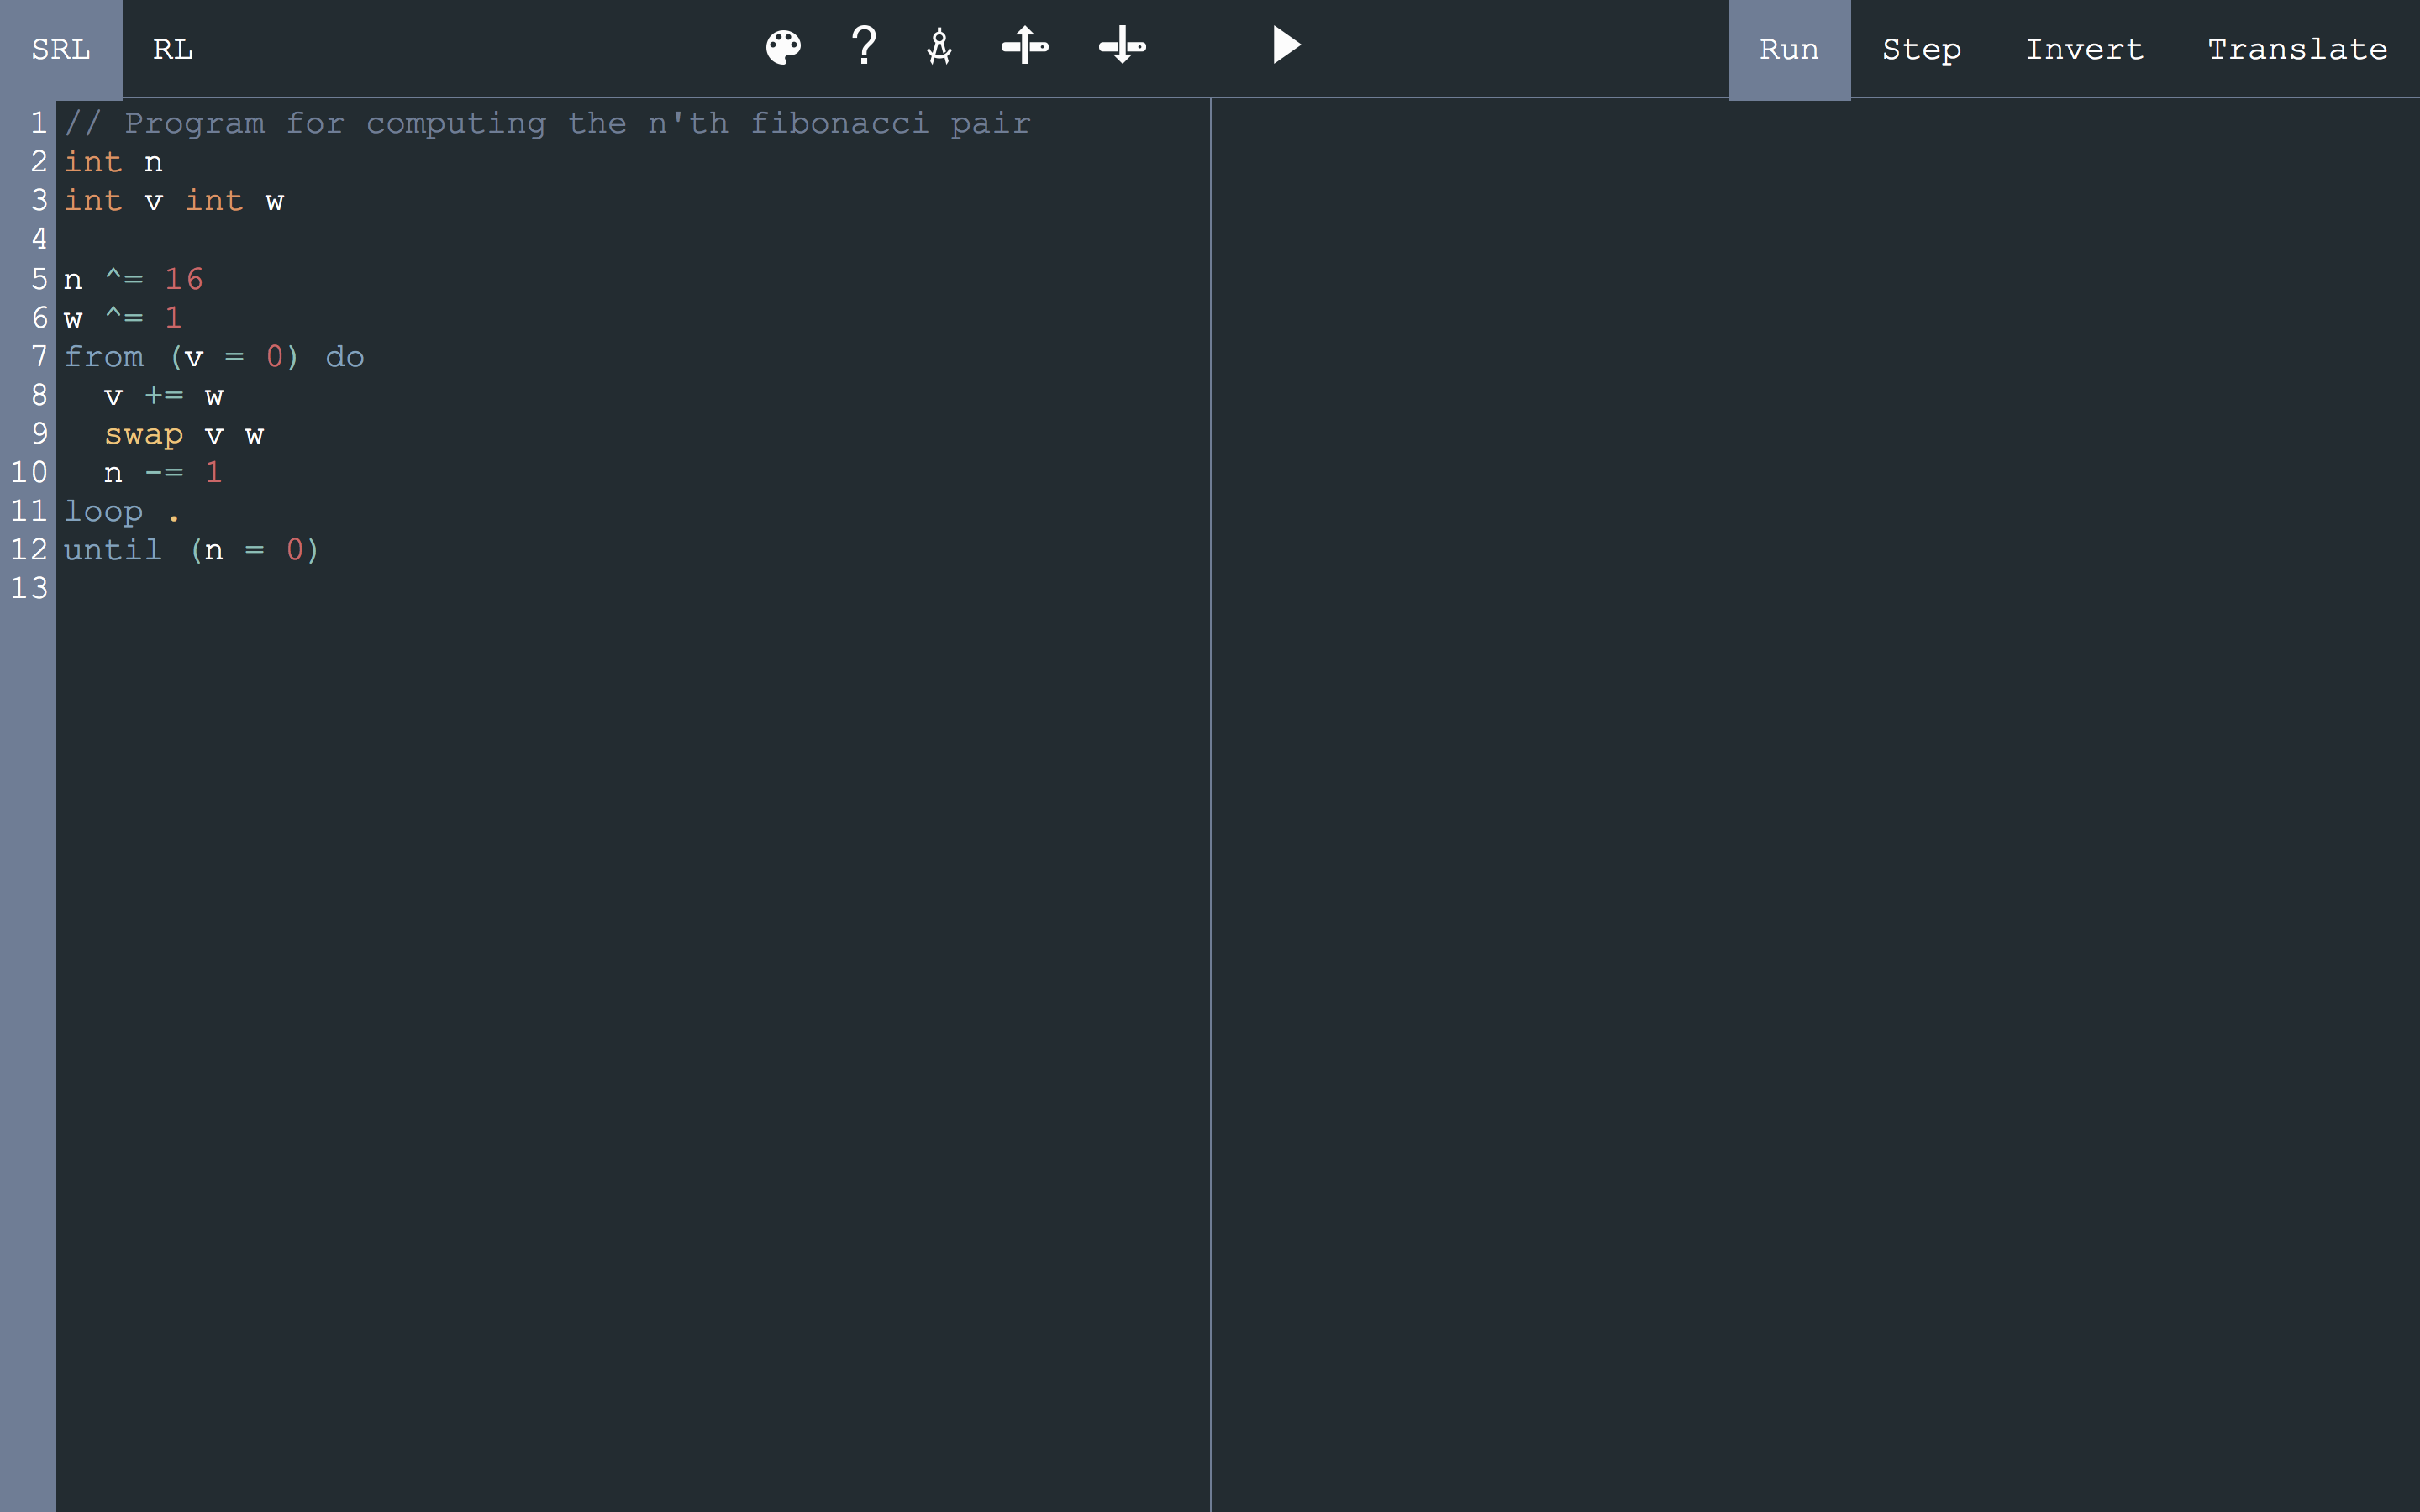
\includegraphics[width=\textwidth]{web_client_ui.png}
%  \caption{Screenshot of web client UI.}
%  \label{fig:web_client_ui}
%\end{figure}

At the far left of the toolbar we have two radio buttons with the options SRL and RL, respectively. The highlighted option indicates how the code in the code editor should be interpreted; if RL is chosen, the code is interpreted as an RL program and similarly, if SRL is chosen, the code is interpreted as an SRL program.

In the middle of the toolbar, above the code editor, we have a group of five icons:
\begin{description}

  \item[\inlineicon{themes.png} Themes]~\\
    By hovering over this icon a dropdown menu, for choosing the color scheme/ theme of the client interface, appears. %This can be seen in Fig.~\ref{app:web_client_themes}.
    %Fig. \ref{fig:web_client_white_ui} shows the color scheme when the white theme is chosen.
    %\begin{figure}
    %  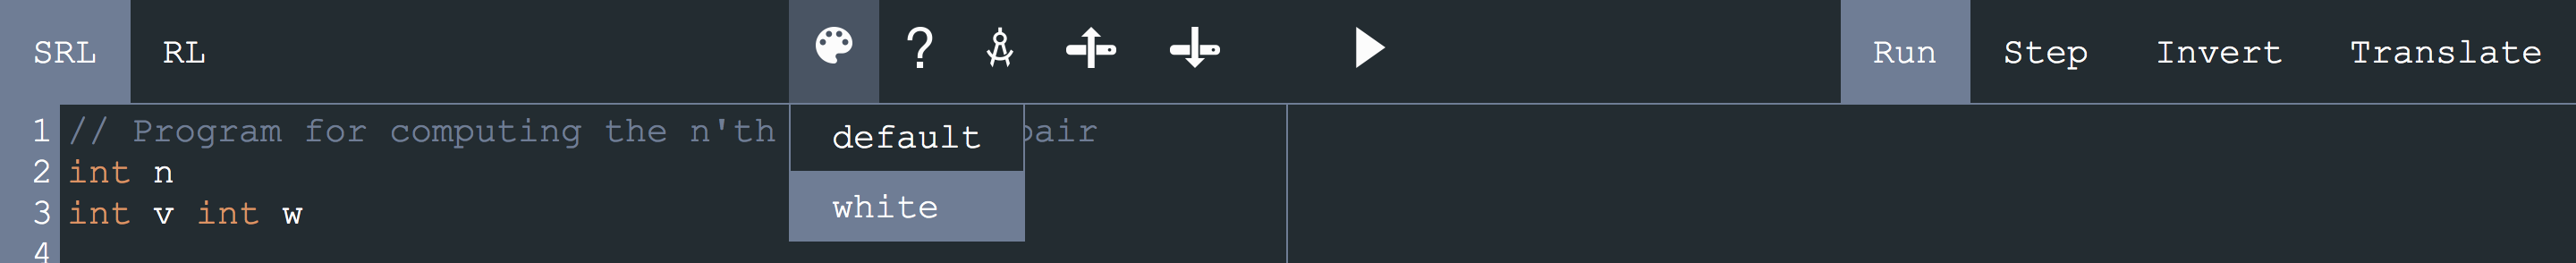
\includegraphics[width=\textwidth]{web_client_themes.png}
    %  \caption{Web client themes dropdown menu.}
    %  \label{fig:web_client_themes}
    %\end{figure}
    %\begin{figure}
    %  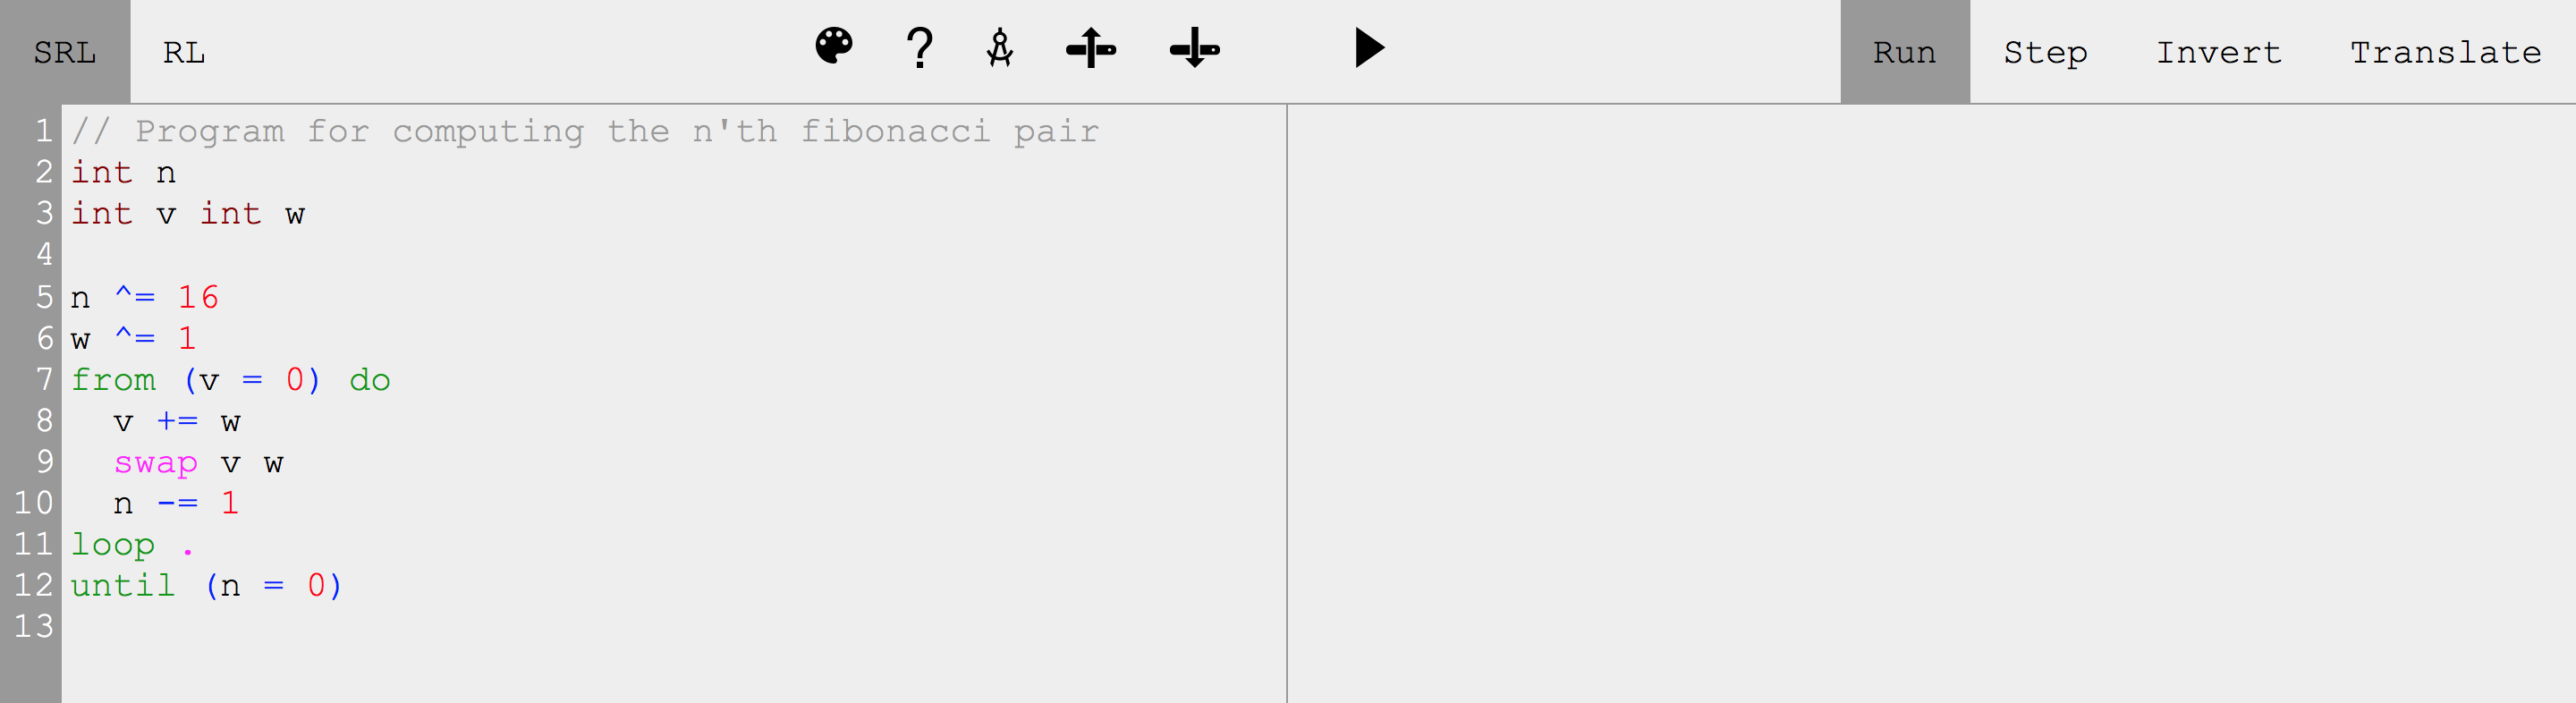
\includegraphics[width=\textwidth]{web_client_white_ui.png}
    %  \caption{Web client UI in white theme color scheme.}
    %  \label{fig:web_client_white_ui}
    %\end{figure}

  \item[\inlineicon{help.png} Help]~\\
    By clicking on this icon a modal window displaying some help text opens. This help text seeks to explain the web interface, the modes and the languages to the user.
    %\begin{figure}
    %  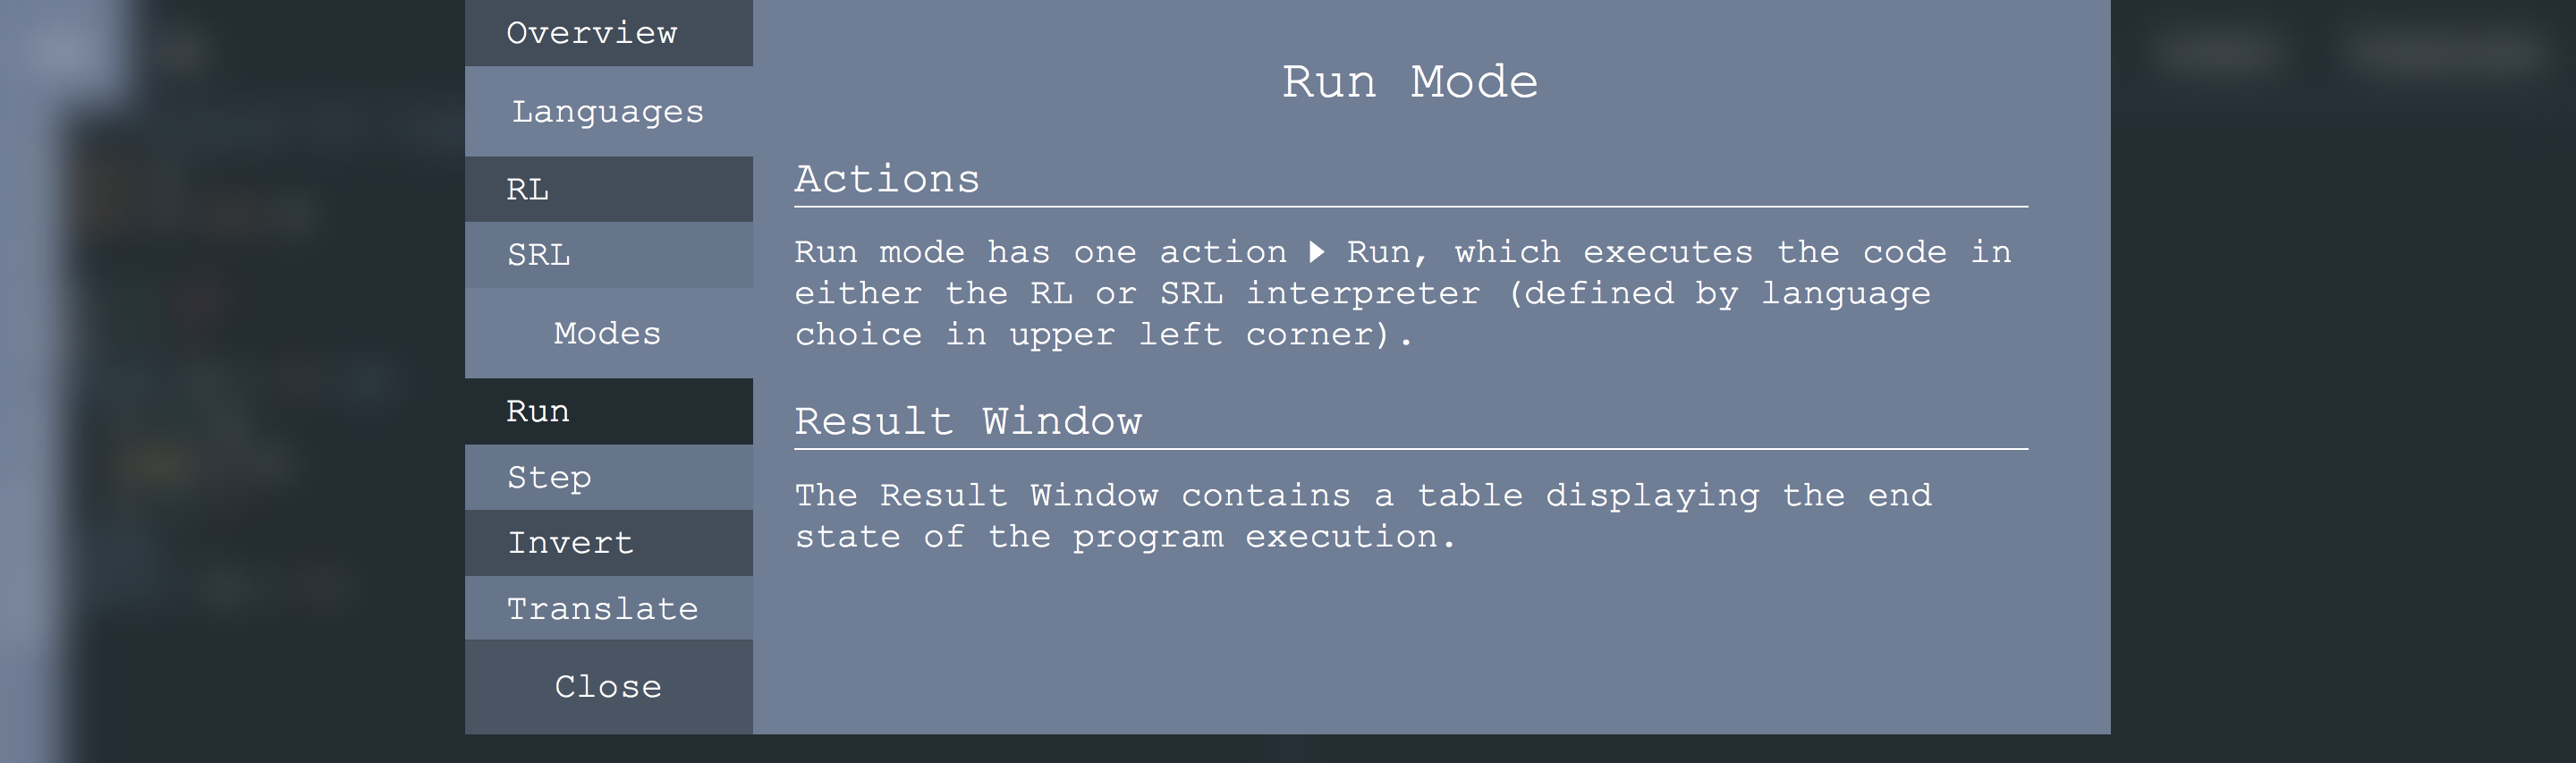
\includegraphics[width=\textwidth]{web_client_help.png}
    %  \caption{Web client help modal window displaying the Run mode help page.}
    %  \label{fig:web_client_help}
    %\end{figure}

  \item[\inlineicon{template.png} Templates]~\\
    By hovering over this icon a dropdown menu appears. This menu contains a series of template programs for both RL and SRL which can be loaded into the code editor.
    %\begin{figure}
    %  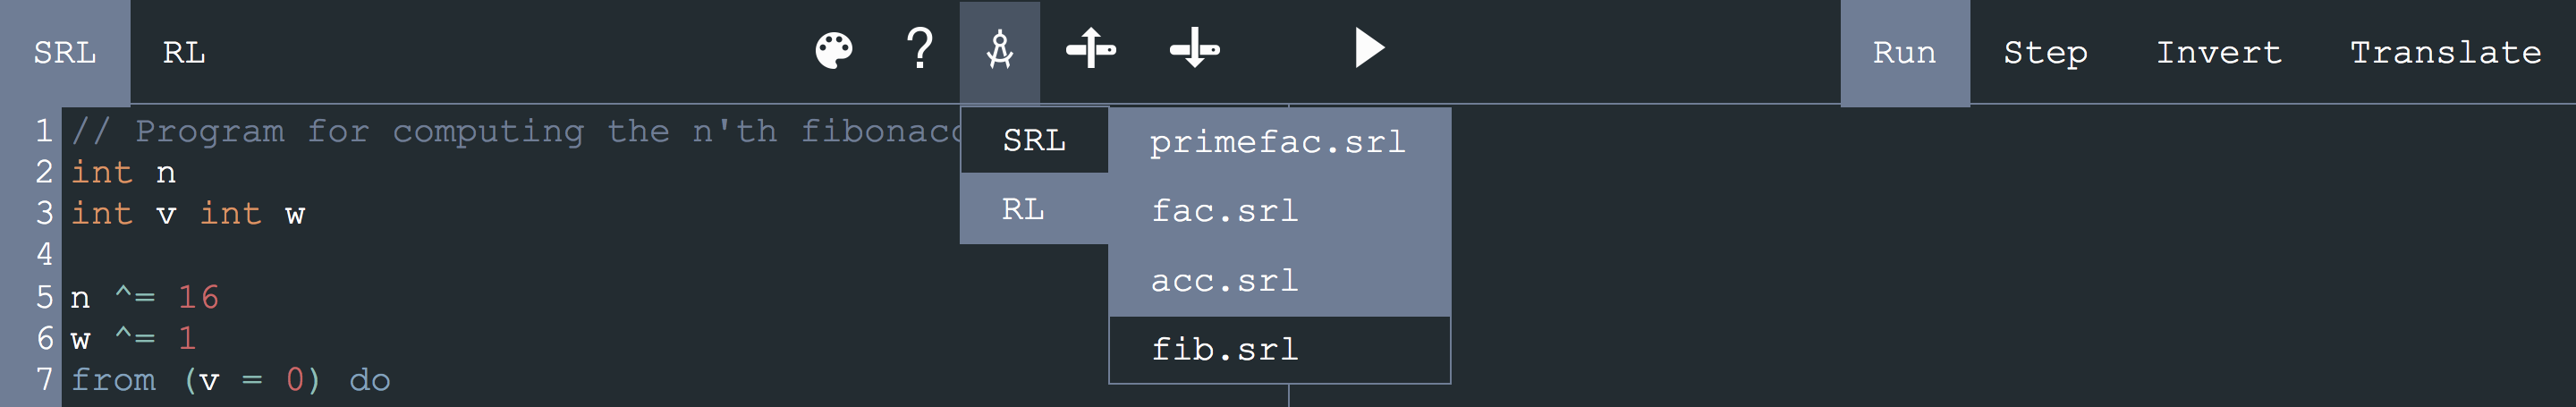
\includegraphics[width=\textwidth]{web_client_templates.png}
    %  \caption{Web client templates dropdown menu.}
    %  \label{fig:web_client_templates}
    %\end{figure}

  \item[\inlineicon{open.png} Open]~\\
    By clicking on this icon a modal window opens. Here it is possible to import and open previously stored programs.
    %\begin{figure}
    %  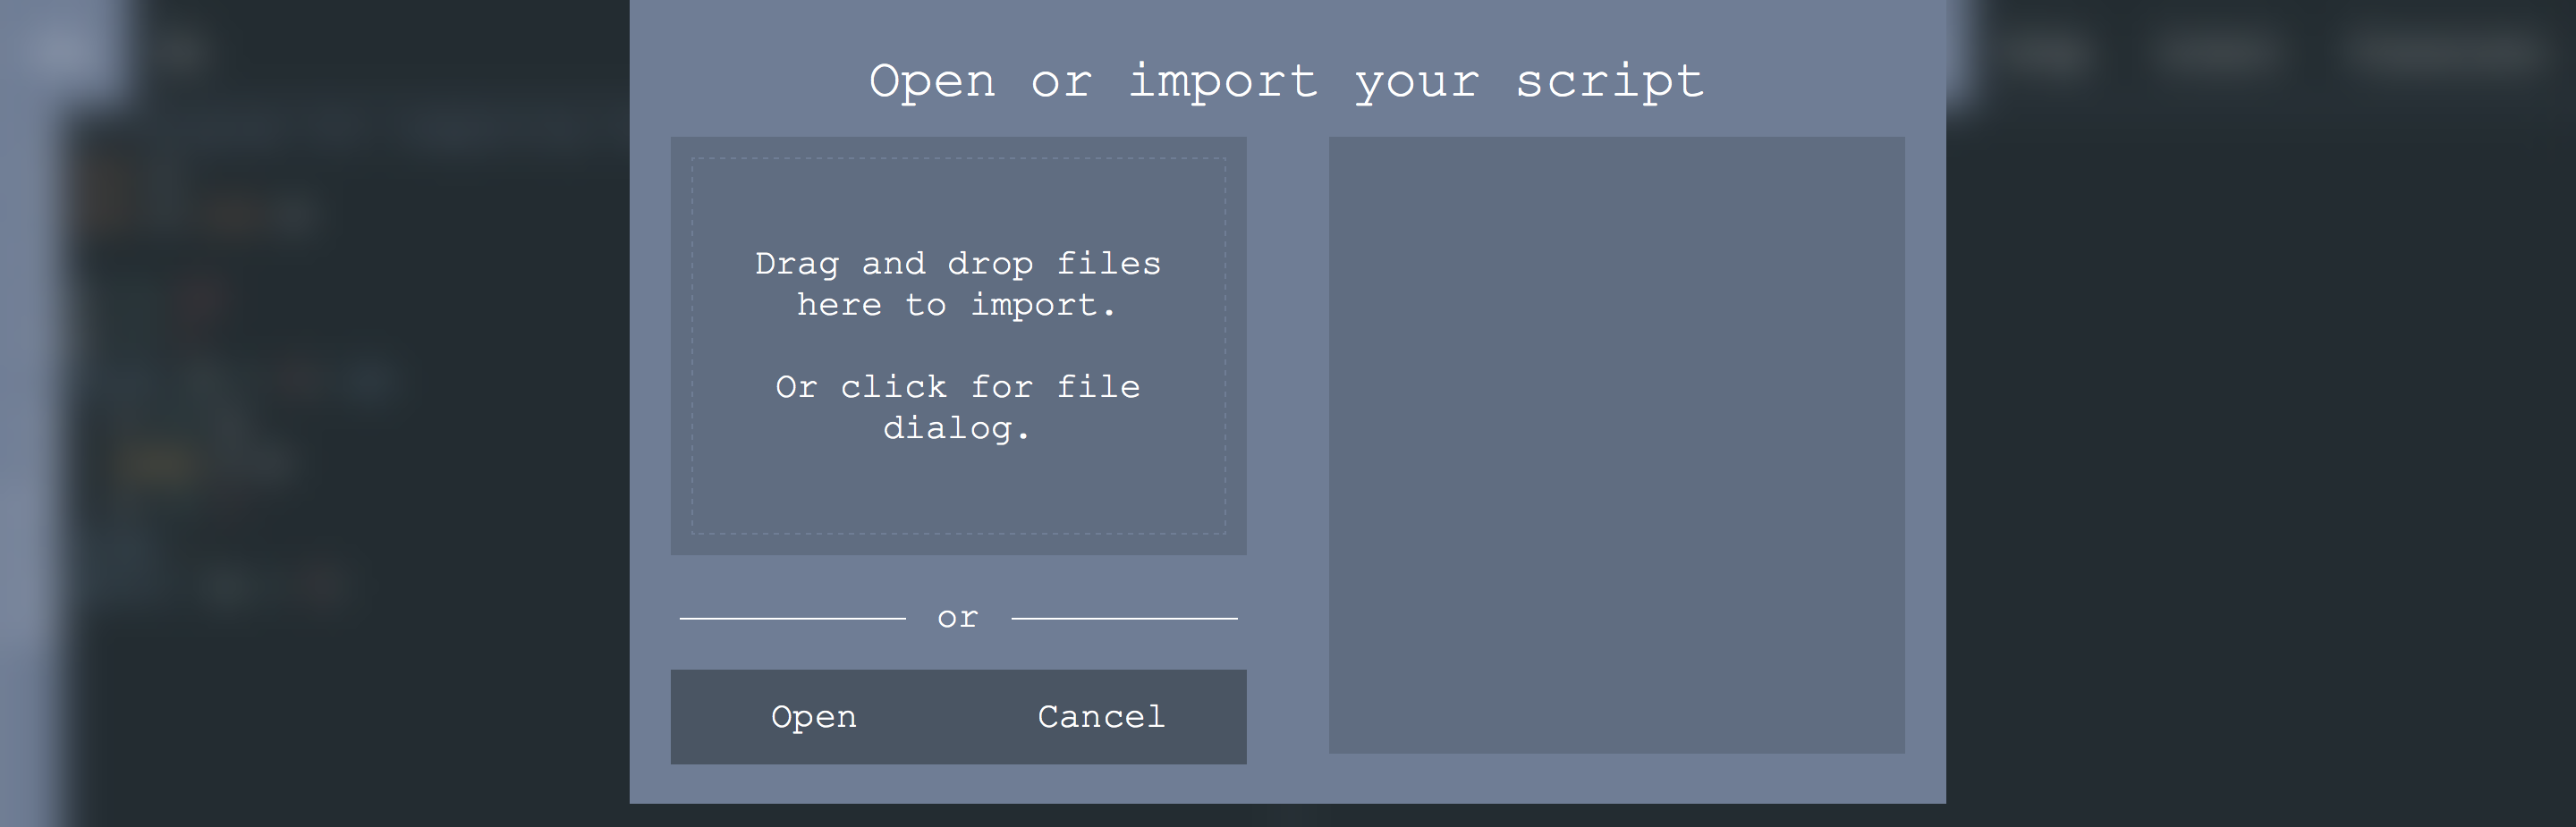
\includegraphics[width=\textwidth]{web_client_open.png}
    %  \caption{Web client open modal window.}
    %  \label{fig:web_client_open}
    %\end{figure}

  \item[\inlineicon{save.png} Save]~\\
    By clicking on this icon a modal window opens. Here it is possible to export, share and store the code currently loaded into the code editor.
    %\begin{figure}
    %  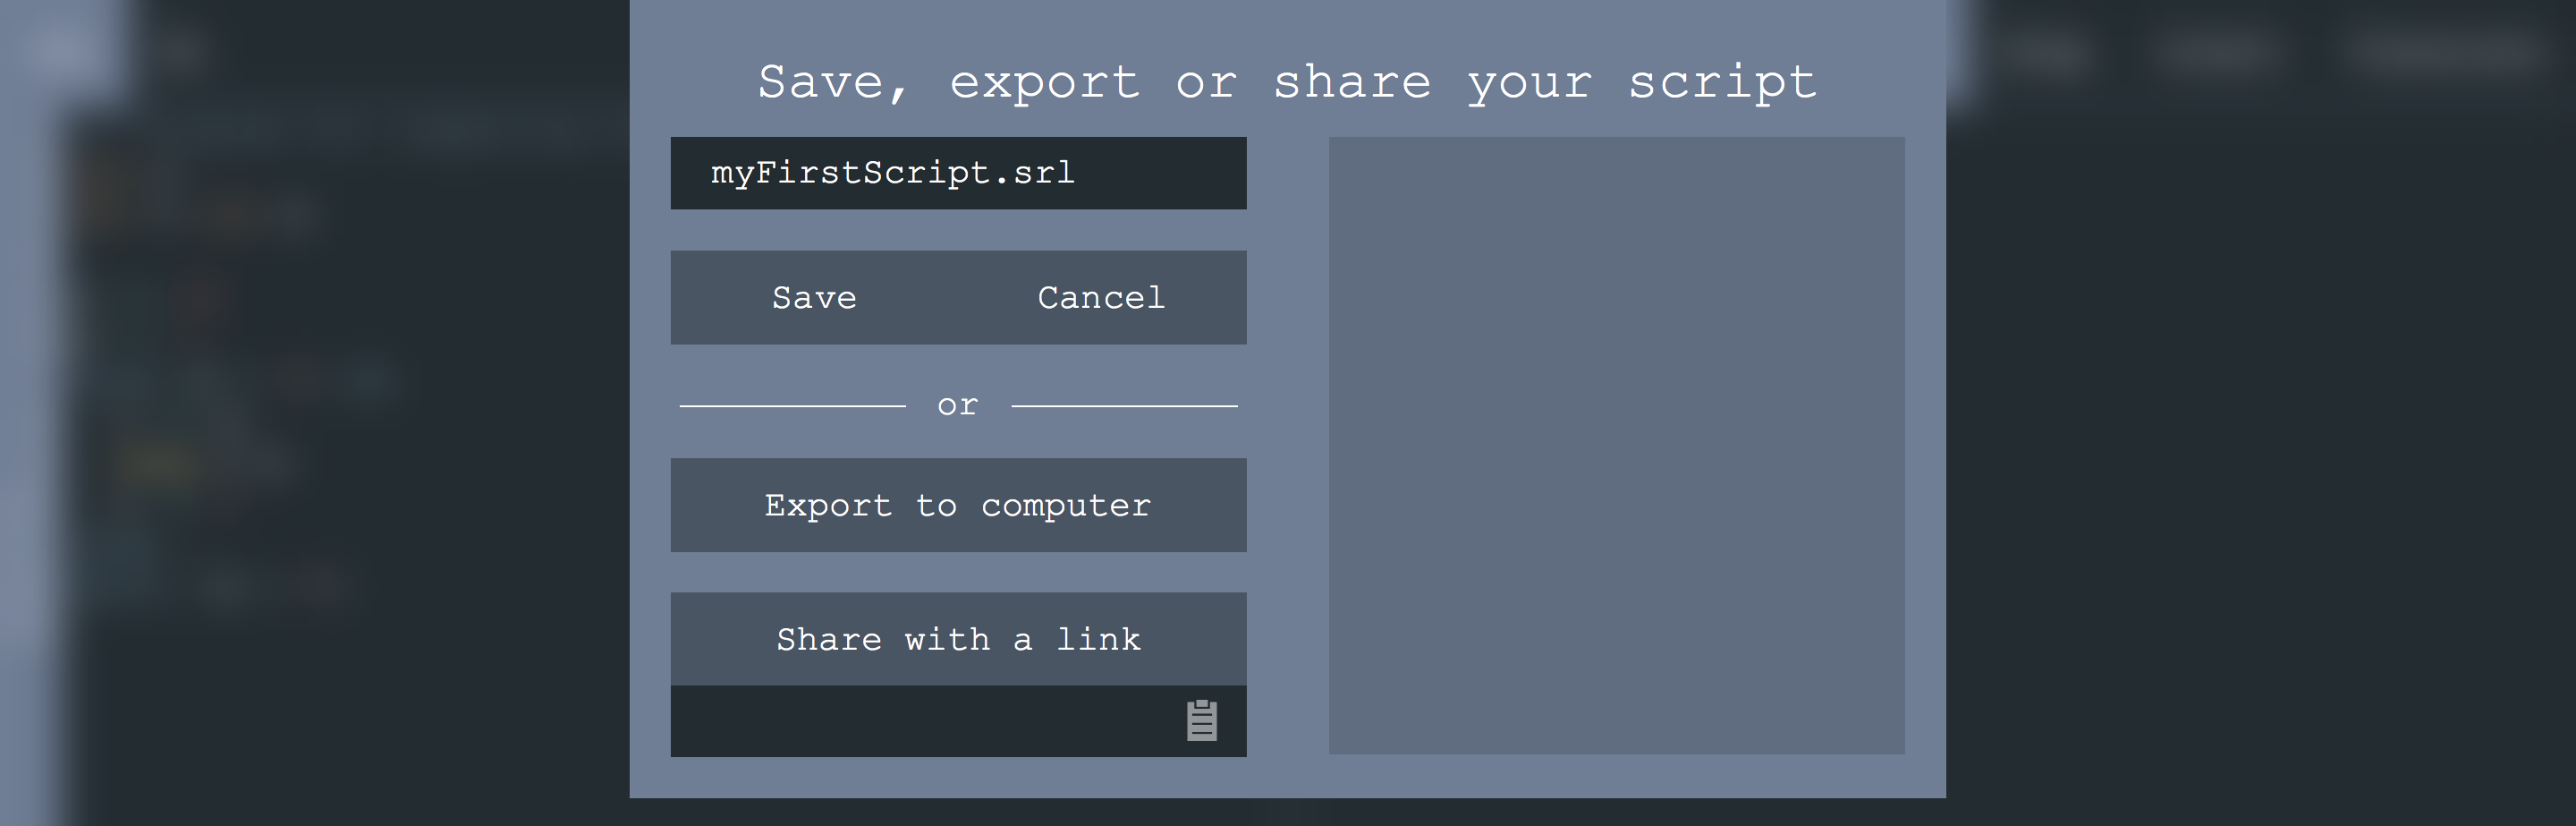
\includegraphics[width=\textwidth]{web_client_save.png}
    %  \caption{Web client save modal window.}
    %  \label{fig:web_client_save}
    %\end{figure}

\end{description}
The right-hand side of the toolbar is dedicated to modes and their associated actions.

There are 4 modes which are selected from the radio button group at the far right:
\begin{description}

  \item[Run]~\\
    The \textit{Run} mode simply executes the code in the editor depending on the chosen language. This is done by clicking \inlineicon{play} \textbf{run}.

  \item[Step]~\\
    The \textit{Step} mode allows for step-by-step program execution. %This even makes for a simple debugger.
    To begin the step-by-step execution, one has to click on \inlineicon{play} \textbf{begin stepping}. Then, the user has five options:
    \inlineicon{prev} \textbf{previous step} undoes the last executed step operation;
    \inlineicon{next} \textbf{next step} executes the next step operation;
    \inlineicon{reset} \textbf{reset} undoes all executed step operations;
    \inlineicon{exec} \textbf{end} executes all remaining step operations;
    \inlineicon{stop} \textbf{stop} stops the execution and leaves the step-by-step execution.
    While in step-by-step execution, all other features are disabled.

  \item[Invert]~\\
    The \textit{Invert} mode simply inverts the code in the editor depending on the chosen language. This is done by clicking \inlineicon{play} \textbf{invert}.

  \item[Translate]~\\
    The \textit{Translate} mode translates the code in the editor depending on the chosen language. This is done by clicking \inlineicon{play} \textbf{translate}.

\end{description}
All the above modes have the ability to fail on a parse- or static error. % Fig. \ref{fig:web_client_error} illustrates a case where a parse error occurs.

%\begin{figure}
%  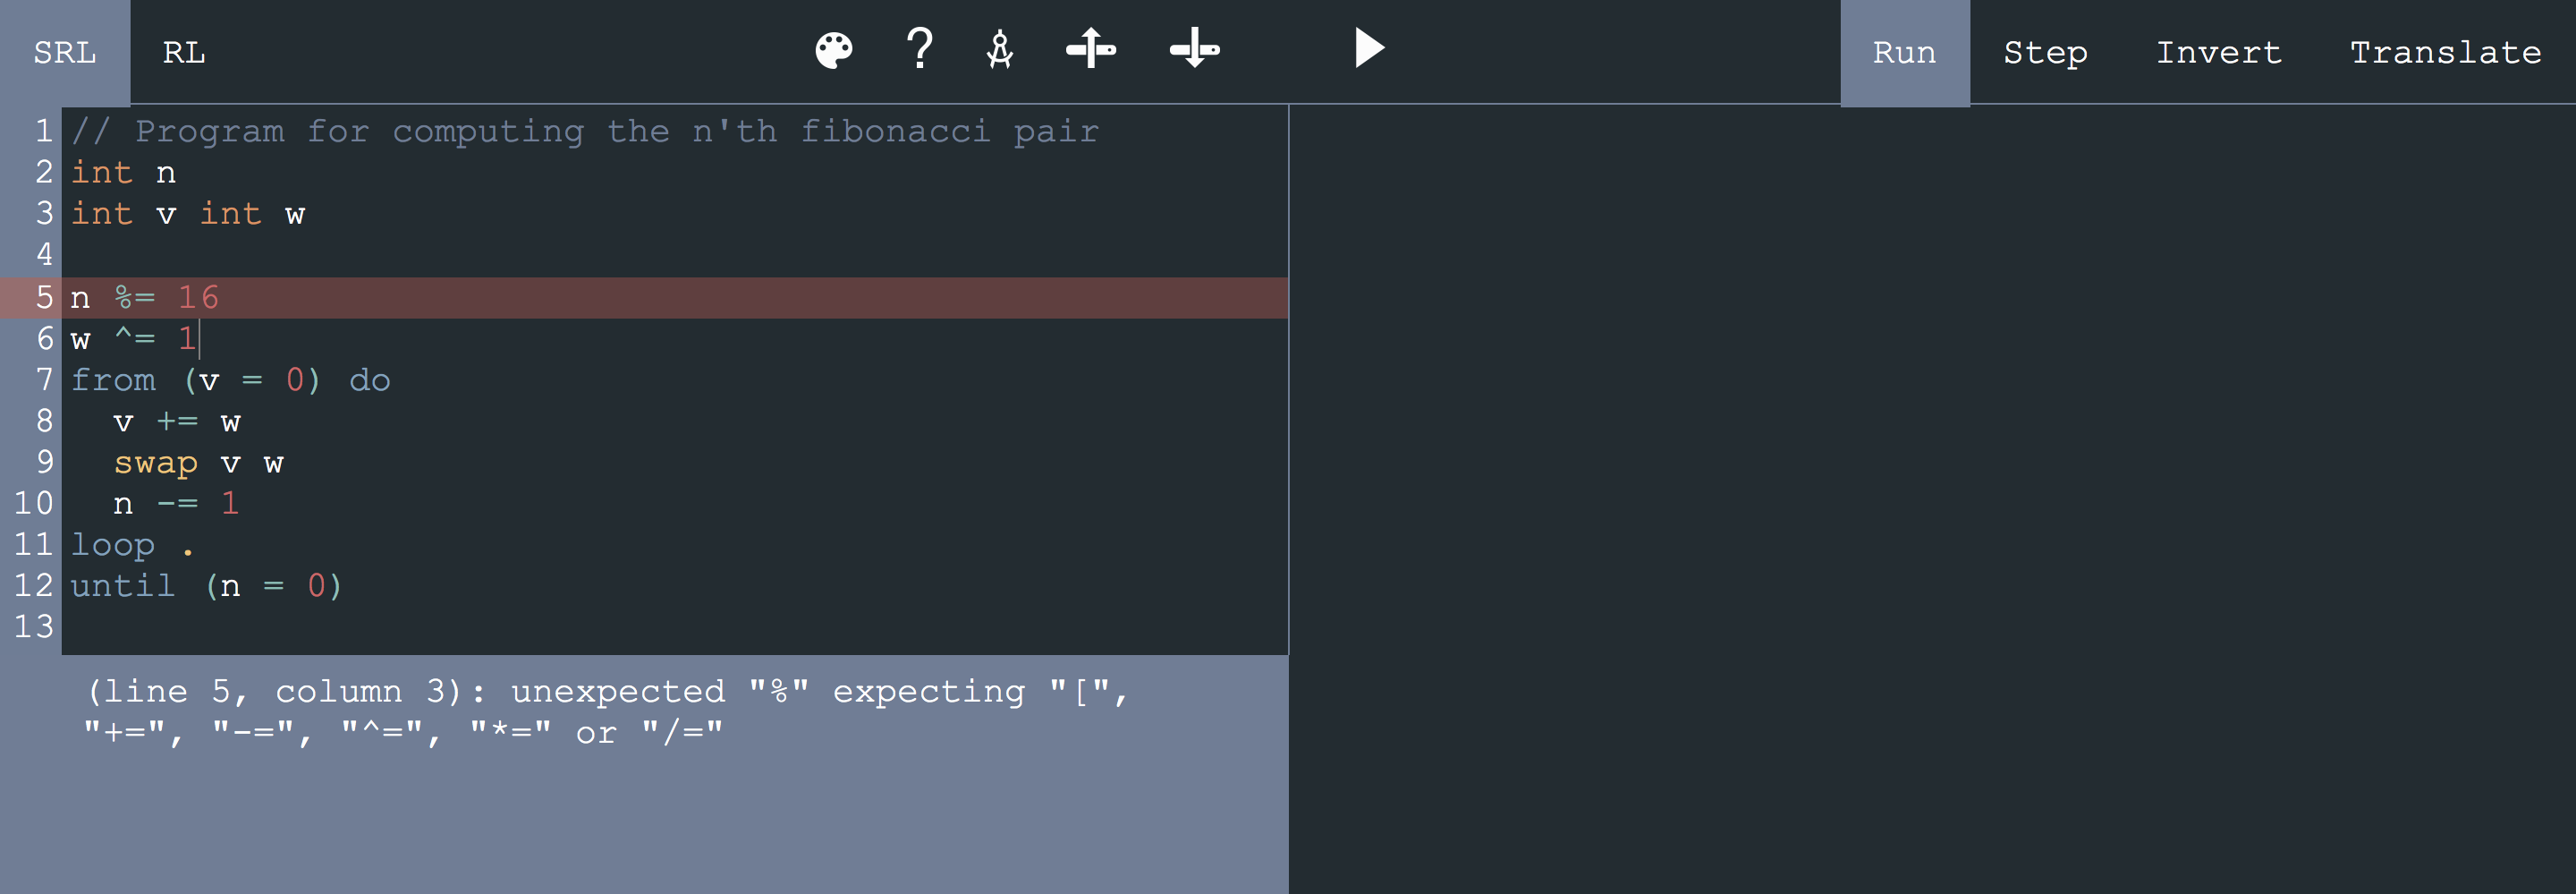
\includegraphics[width=\textwidth]{web_client_error.png}
%  \caption{Web client with parse error.}
%  \label{fig:web_client_error}
%\end{figure}

%%%%%%%%%%%%%%%%%%%
%%% Implementation
%%%%%%%%%%%%%%%%%%%

\subsubsection{Implementation}

Now that the features have been introduced, we can briefly look at the implementation.
The web client interface is a nodeJS project written in ECMAScript 6, using the library ReactJS, for creating modularised components.
We chose to use ReactJS instead of vanilla javascript and html, since it allows component rendering based on state.
This way focus was primarily on state and logic instead of design and propagating state to the application.
To separate state and logic from UI even further, we chose to handle state through Redux.
This way we could move state and alteration of state outside of the ReactJS components, hereby giving the individual components access to only the absolute necessary state variables and state alterations methods. Thus, the possibilities of a specific state alteration failing are limited to the components with access which, in turn, makes it easier to debug and fix.

The web client interface uses babel and webpack to compile and bundle scripts and resources.
Webpack uses babel to convert JSX to React components and transpile ECMAScript 6 to ECMAScript 5 in order to allow for \texttt{import} statements.
Webpack itself is used to precompile SASS, which is used for styling, to CSS, appending prefixes to the CSS for better cross-browser support and bundling scripts, styles and assets for minimal HTTP requests.

The root of the web client is \path{/web/client}. Configuration files for node package dependencies and the webpack build flow are found here.
Under the subdirectory \path{src/} are all source files and resources located.
ReactJS components are found under \path{src/components} and the corresponding styling/ SASS files are found under \path{src/styles} along with the theme color schemes in the subdirectory \path{src/styles/themes}.

The root component is the \textit{App} component which contains all the major components as children.
The App component is wrapped in a redux provider which allows the app and all its children access to the application state and state modifiers.
The children components of the App component are:
\begin{description}

  \item[Header]~\\
    Utilises the Button, Radio and Dropdown components for letting the user interact with the application.

  \item[Editor]~\\
    The editor has two areas; the coding area, which is visible at all times, and the error area, which only is visible when an error is present.
    The code editor component is the javascript library CodeMirror \cite{CM} delivered through the react-wrapper React CodeMirror 2.
    CodeMirror was chosen since it has a library for lexing --- used for syntax highlighting --- along with a lot of customisation options and extendibility through plugin support.

  \item[Result]~\\
    The result area presents the the potential results of the actions associtated with a mode. A program state is displayed as a lists of values, a step log (under the Step mode --- is displayed as a list of individual step operations, and program transformations are displayed through a read-only CodeMirror instance.

  \item[Modals]~\\
    `Modals` covers the HelpModal, OpenModal and SaveModal components, which use the same Button, Radio and Dropwdown components as the Header.

\end{description}
For more information regarding the implementation, refer to the source code in Appendix \ref{app:web_client}.



\subsection{Server \& API}
\label{sec:server_and_api}

The web server is an independent node project which, when built, uses the client web interface and the command-line interfaces as dependencies.
These are built and copied into the web server project folder.
The command-line interface binaries are placed under \path{/web/server/bin} and the web client interface is placed under \path{/web/server/client}.

The server is written in ECMAScript 6, but since nodeJS (version 9 and below) does not support \texttt{import} statements natively, the Babel transpiler is used for running the ECMAScript 6 code as ECMAScript 5.
This is done in the entry-file \path{babel-server.js}, as a wrapper for the actual server configuration in \path{server.js}.
We run the transpiled code with node and use the Express package for opening ports, setting up the server and handling web-routes.
All communication between the API server and the client-side is formatted as JSON; as are the results from the command-line interfaces.
This way it is easy to parse data from the interpreter to the client interface via the API.

The server has Cross Origin Resource Sharing (CORS) enabled, to allow for separation of the API server and the client web interface.
This allows for the server to be hosted at one address, while the interface is hosted at another.
CORS is enabled by setting the appropriate headers. That is,
\lstinputlisting[language=javascript,firstline=10,firstnumber=10,lastline=15]{../web/server/server.js}
The routing has two responsibilities: to handle API calls, which can be seen in Fig. \ref{fig:full_api}, and to serve static files when the client interface is requested. The defined routes are listed in Fig. \ref{fig:server_routes}. Routes are divided into 3 categories: API routes, root requests and static files; where static files are the bundled css and javascript files that the client interface requires.
If the client interface is hosted at a different address than the API, the \path{/web/server/client} folder can be removed, causing the route for the index page and the static pages to respond with a 404 (page not found) status and page.
In this case, to get the client to point to the correct API address, change the API\_URL found variable in \path{/web/client/webpack.prod.config.js} and rebuild the client interface.

The API sub-URLs, along with their valid request method(s) and functionality, are described in Fig. \ref{fig:full_api}.
\begin{figure}
  \begin{tabular}{|l|l|p{6.7cm}|}\hline
    \textbf{Route} & \textbf{Method} & \textbf{Responsibility}\\\hline
    \texttt{/run/:language} & \texttt{POST} & Here \texttt{:language} can either be \texttt{rl} or \texttt{srl}.
                                                This API-call executes the code that is posted along with the request, and returns the end-state of the program.
                                                The code submitted should be wrapped in a JSON object, with the attribute \texttt{code}.\\\hline
    \texttt{/run/log/:language} & \texttt{POST} & Is equivalent to \texttt{/run/:language}, but instead of returning the end-state
                                                    alone, it also returns the json-formatted execution-log.\\\hline
    \texttt{/invert/:language} & \texttt{POST} & Here \texttt{:language} can either be \texttt{rl} or \texttt{srl}.
                                                This API-call inverts the code.
                                                The code submitted should be wrapped in a JSON object, with the attribute \texttt{code}.\\\hline
    \texttt{/translate/:language} & \texttt{POST} & Here \texttt{:language} can either be \texttt{rl} or \texttt{srl}.
                                                This API-call translates the code from the specified language to its counterpart.
                                                The code submitted should be wrapped in a JSON object, with the attribute \texttt{code}.\\\hline
    \texttt{/template/list}  & \texttt{GET} & Returns a list of SRL and RL files, as a JSON-object. The object has the attributes \texttt{srl} and \texttt{rl}, where each corresponding value is a list of template-names for that language. \\\hline
    \texttt{/template/:file} & \texttt{GET} & Here \texttt{:file} is the template requested.
                                              A JSON-object, with the attribute \texttt{code}, which contains the code of the requested template file, is returned.\\\hline
  \end{tabular}
  \caption{API routes.}
  \label{fig:full_api}
\end{figure}
\begin{figure}
  \begin{tabular}{|l|p{8.7cm}|}\hline
    \textbf{Route} & \textbf{Responsibility}\\\hline
    \texttt{/}     & Fetch the built client interface index page from \path{/web/server/client/index.html}.\\\hline
    \texttt{/api*} & Here \texttt{*} is everything after \texttt{/api}, which is forwarded to the API router. The API routes are described in Fig. \ref{fig:full_api}. \\\hline
    \texttt{/:filename.:ext}     & Here \texttt{:filename.:ext} matches a static resource, e.g. \texttt{bundle.js}. All static files are fetched from \path{/web/server/client}. Thus only files that the client interface uses can be requested.\\\hline
  \end{tabular}
  \caption{Routes for web server.}
  \label{fig:server_routes}
\end{figure}

For accessing the command-line interfaces and fetching template files, the interface \texttt{execFile(file, [arguments], callback)} from the node module child\_process is used.
\texttt{execFile} takes the arguments to the file as a list, where each element is treated as one argument.
Instead of opening a shell and calling the file, execFile executes the file directly, which disallows for injections such as '" \&\& ls \#' for getting information about the host system.

% \begin{lstlisting}[language=javascript]
% execFile(cmd,
%         [mode, code, flags],
%         {maxBuffer, timeout},
%         (err, stdout, stderr) => {
%   // ... callback content
% });
% \end{lstlisting}


\section{Further Improvements}

\subsection{Interpretation}

\todo{faster interpretation, optimising the code}

\subsection{Parsing}

\todo{not ignoring newlines, generates better error messages and allows more syntactic sugar}

\subsection{Optimisation}
\todo{Talk about zippers with a reference}
\todo{Graph AST for RL?}
\todo{Better use of typeclasses/other?}

\todo{optimisation of Common: merge updates, compute constants, remove redundant stuff, remove skips}
\todo{optimisation of RL: AST as a cyclic graph, reduce the graph}

\subsection{Web}
\todo{API-keys}

